%
% Monografia apresentada à
% Escola Politécnica da Universidade de São Paulo
% documentando o trabalho de conclusão do curso
% de Engenharia Elétrica com ênfase em Computação,
% desenvolvido no decorrer do ano de 2010.
%
% Autores
% -------
% Murilo Cerone do Nascimento
% Tássio Naia dos Santos
%
% Trabalho orientado por
% ----------------------
% Ricardo Nakamura
% Roberto Bianchini
%

\documentclass[a4paper,12pt]{report}

\usepackage{comment} % para ``esconder'' coisas...

\usepackage[brazilian,english]{babel}
\usepackage[utf8]{inputenc}
\usepackage{a4wide}
\usepackage[section]{placeins}
\usepackage{txfonts}
\usepackage{type1cm}
\usepackage{courier}
\usepackage[scaled]{helvet}
\usepackage{epigraph}
\renewcommand*\familydefault{\sfdefault}

\hyphenation{
  es-ta-be-le-ci-do
  a-de-qua-da-men-te
  pro-ble-mas
  di-men-sio-na-men-to
  mo-de-lo
}

% Controlar linhas orfas e viuvas
\clubpenalty=10000
\widowpenalty=10000
\displaywidowpenalty=10000

% Formatar notas de rodape
\usepackage[hang]{footmisc}
\setlength{\footnotemargin}{1em}

\usepackage{url}
%% Define a new 'leo' style for the package that will use a smaller font.
\makeatletter
\def\url@leostyle{%
  \@ifundefined{selectfont}{\def\UrlFont{\sf}}{\def\UrlFont{\small\ttfamily}}}
\makeatother
%% Now actually use the newly defined style.
\urlstyle{leo}

\usepackage[left=3cm,top=3cm,right=2cm,bottom=2cm,includehead,ignoremp]{geometry}

\usepackage[small]{titlesec}
% \titlespacing{\chapter}{0pt}{-50pt}{*20}[0pt]
\titlespacing{\chapter}{0pt}{*-10}{*5}

% Running Headers and footers
\usepackage{fancyhdr}
% \pagestyle{fancy}
\pagestyle{headings}
% Redefine plain page style
\fancypagestyle{plain}{
  \fancyhf{}
  \renewcommand{\headrulewidth}{0pt}
  \fancyhead[LE,RO]{\thepage}
}

\linespread{1.3}
%\pdfpagewidth=\paperwidth
%\pdfpageheight=\paperheight

% Para habilitar cálculos em dimensões
\usepackage{calc}

% Multipart figures
%\usepackage{subfigure}

% More symbols
%\usepackage{amsmath}
%\usepackage{amssymb}
%\usepackage{latexsym}

% Surround parts of graphics with box
\usepackage{boxedminipage}

% Package for including code in the document
\usepackage{listings}

% If you want to generate a toc for each chapter (use with book)
%\usepackage{minitoc}

% This is now the recommended way for checking for PDFLaTeX:
\usepackage{ifpdf}

\ifpdf
\usepackage[pdftex]{graphicx}
\else
\usepackage{graphicx}
\fi

%% Parece que essas informações não são usadas
\title{Arquitetura \empb{BDI} para agentes e \emph{Blackboard}: um
  estudo de caso de técnicas de Inteigência Artificial aplicadas a jogos}
\author{Murilo Cerone doNascimento \\ murilo.cerone@gmail.com \ands
Tássio Naia dos Santos \\ tassio.naia@gmail.com %\and
%Beltrano \\ beltrano@gmail.com
}
\date{2010-10-5}

\usepackage[absolute]{textpos}

% Comandos
% --------
% Abreviações
\newcommand{\npc}{\textsc{npc}}

\begin{document}

\ifpdf
\DeclareGraphicsExtensions{.png, .pdf, .jpg, .tif}
\else
\DeclareGraphicsExtensions{.eps, .jpg}
\fi


\pagestyle{empty}
\pagestyle{empty}
\begin{center}
  {\large Murilo Cerone do Nascimento \\
    Tássio Naia dos Santos}
\end{center}

\begin{textblock*}{21cm}[0,0](0cm,12cm)
  \begin{center}
    {\LARGE Arquitetura \emph{BDI} para agentes e \emph{Blackboard}:\\
      um estudo de caso de técnicas de IA aplicadas a jogos}
  \end{center}
\end{textblock*}


\begin{textblock*}{21cm}[0,0](0cm,29.7cm-4cm)
  \begin{center}
    {\large São Paulo \\ 2009 }
  \end{center}
\end{textblock*}



\newpage
\begin{center}
  {\large Murilo Cerone do Nascimento \\
    Tássio Naia dos Santos}
\end{center}

\begin{textblock*}{21cm}[0,0](0cm,12cm)
  \begin{center}
    {\LARGE Arquitetura \emph{BDI} para agentes e \emph{Blackboard}:\\
      um estudo de caso de técnicas de IA aplicadas a jogos}
  \end{center}
\end{textblock*}


\begin{textblock*}{21cm}[0,0](0cm,29.7cm-4cm)
  \begin{center}
    {\large São Paulo \\ 2009 }
  \end{center}
\end{textblock*}




\begin{textblock*}{21cm/2-2cm}[0,0](21cm/2,15cm)
  \begin{flushleft}
    {\large
  Monografia apresentada à Escola Politécnica da Universidade de São Paulo para obtenção do título de Bacharel em Engenharia.\newline
  \newline
  Área de Concentração:\newline
  Engenharia de Computação\newline
}


  \end{flushleft}
\end{textblock*}



\begin{center}
  {\large Murilo Cerone do Nascimento \\
    Tássio Naia dos Santos}
\end{center}

\begin{textblock*}{21cm}[0,0](0cm,12cm)
  \begin{center}
    {\LARGE Arquitetura \emph{BDI} para agentes e \emph{Blackboard}:\\
      um estudo de caso de técnicas de IA aplicadas a jogos}
  \end{center}
\end{textblock*}


\begin{textblock*}{21cm}[0,0](0cm,29.7cm-4cm)
  \begin{center}
    {\large São Paulo \\ 2009 }
  \end{center}
\end{textblock*}




\begin{textblock*}{21cm/2-2cm}[0,0](21cm/2,15cm)
  \begin{flushleft}
    {\large
  Monografia apresentada à Escola Politécnica da Universidade de São Paulo para obtenção do título de Bacharel em Engenharia.\newline
  \newline
  Área de Concentração:\newline
  Engenharia de Computação\newline
}



    {\large
      Orientadores:\newline
      Ricardo Nakamura\newline
      Roberto Cezar Bianchini
    }
  \end{flushleft}
\end{textblock*}


\begin{textblock*}{21cm/3}[0,0](21cm/3*2-2cm,29.7cm-6cm)
  \begin{flushright}
    {\emph{
      \`All you need is love...}
    }
  \end{flushright}
\end{textblock*}

\null\newpage



% agradecimentos (opcional)
%\epigraph{``Pequenas oportunidades são muitas vezes o começo de grandes empreendimentos.''}{Demóstenes\\Político e pensador grego\\(384 a.C. - 322 a.C)}

\epigraph{``O resultado de qualquer pesquisa séria só pode ser fazer
duas questões crescerem onde antes só crescia uma.''}{Thorstein
Veblen\\Sociólogo e economista noruego-estadunidense\\(1853 -- 1929)}


\pagenumbering{roman}

% Resumo e Abstract
\selectlanguage{brazilian}
  \begin{abstract}
    Esta monografia aborda o desenvolvimento de um estudo de caso do emprego de técnicas de inteligência artificial a um jogo. Neste estudo foram aplicadas a arquitetura \emph{Belief--Desire-Intention} (BDI) para agentes cognitivos e a técnica blackboard (para compartilhamento de conhecimento entre agentes) de modo a enriquecer a complexidade e variabilidade de reação do jogo e seus \emph{non-controlled players} (\npc{}s). Foram considerados aspectos da eficiência do uso de um interpretador de linguagem de programação orientada a agentes, em conjunto com um sistema de renderização e controle da lógica do jogo compilado.

O trabalho permite observar o ganho de flexibilidade que o emprego de tais técnicas pode agregar ao design de jogos, bem como as limitações técnicas e que decorrem do crescimento de complexidade de modelagem à medida que se multiplicam as escolhas e contextos com os quais lidam os agentes.

Conclui-se que mesmo jogos de pequeno porte podem se beneficiar da agregação de \emph{inteligência artificial} às interações com \npc{}s.


\begin{comment}
Avanços tecnológicos permitem que cada vez mais detalhes e complexidade interajam em jogos.

Com frequência, IA é usada

Agentes Inteligentes. -> tópico da moda
“Agentes de software ou sistemas multi-agentes tem recentemente atraído uma considerável atenção da indústria de software. O objetivo deste capítulo é introduzir este novo paradigma de desenvolvimento que é adequado para o desenvolvimento de complexos sistemas de software. Debateremos porque que a abordagem orientada a agente é um genuíno avanço em relação ao estado da arte. Uma visão geral dos principais conceitos, métodos e ferramentas existentes é apresentada. Descreveremos em detalhe o framework Tropos. Os principais desafios do paradigma de agentes para o desenvolvimento de software são discutidos.
[ JAI ] - Livro das Jornadas de Atualização em Informática
2006 jul. 17-20 : Campo Grande - MS - ISBN 85-87926-19-5
descrição
SEGUNDO ISBN:
TÍTULO: 	ATUALIZAÇÕES EM INFORMÁTICA
ORGANIZADOR: 	KARIN BREITMAN
ORGANIZADOR: 	RICARDO ANIDO
Nº DE EDIÇÃO: 	1
ANO DE EDIÇÃO: 	2006
TIPO DE SUPORTE: 	PAPEL
PÁGINAS: 	464
EDITORA: 	PUC-RIO


”

Falar da motivação para uso de técnicas de IA em jogos, e do potencial
que o BDI e a técnica blackboard têm de agregar ao realismo da experiência
dos jogos. (Citar artigos falando do emprego dessas técnicas.)

Falar do intuito do estudo de caso, do que se pretende (e como)
quantificar. Mencionar as maiores escolhas e como imaginamos que elas
delinearam os resultados. (E instigar o leitor à leitura do restante
da tese!)


% Exemplo de resumo --- muito bom!
\begin{comment}
Numa série de artigos publicados entre 1843 e 1844, M.Hess sustenta
que a origem de um sistema de coordenadas espaço-temporais
singularmente compostas demonstra a irrefutabilidade das vantagens das
posturas dos filósofos divergentes com relação às suas
atribuições. Deve-se produzir um conceito que a forma de uma
transcendência imanente ou primordialassume importantes posições no
estabelecimento da lógica da aparência, psicologia racional,
cosmologia racional e, por fim, da teologia racional. Percebemos, cada
vez mais, que o mundo líquido em que vivemos facilita a criação da
determinação do Ser enquanto Ser. Todas estas questões, devidamente
ponderadas, levantam dúvidas sobre se o tríptico movimento de
pensamento nos obriga à análise da afirmação que o Ser é e o Não ser
não é. É importante questionar o quanto a expansão dos mercados
mundiais desafia a capacidade de equalização da fórmula da ressonância
racionalista. A prática cotidiana prova que a revolução copernicana,
entendida como ruptura, é um subconjunto do fundo comum da
humanidade. Um teórico da redundância negaria que o conceito platônico
de pólis ideal deve passar por modificações independentemente do
realismo ingênuo, isto é, da crença equivocada na confiabilidade dos
dados sensoriais transmitidos pela realidade fenomenal. Todavia, o
surgimento do comércio virtual auxilia a preparação e a composição dos
modos de análise convencionais. Ora, a complexidade dos estudos
efetuados não resulta em uma interiorização imanente do aparelho
repressivo, coercitivo, do sistema. Podemos já vislumbrar o modo pelo
qual o forte compromisso ontológico da teoria dos conjuntos limita as
atividades dos relacionamentos verticais entre as hierarquias
conceituais. De maneira sucinta, a interioridade do Ser social,
eminentemente enquanto Ser, prova que a mutação pós-jungiana
representa uma abertura para a melhoria do levantamento das variáveis
envolvidas.

\end{comment}
% Acho que em algum lugar me disseram que as palavras-chave devem vir
% do pessoal da biblioteca. Mas é possível que eu esteja só me
% confundindo com algum campo da ficha catalográfica...
Palavras-chave: Engenharia. Engenharia da Computação. Inteligência
Artificial. Arquitetura BDI. Sistema Blackboard. Jogos.

  \end{abstract}
\begin{otherlanguage}{english}
  \begin{abstract}
    Numa série de artigos publicados entre 1843 e 1844, M.Hess sustenta que a origem de um sistema de coordenadas espaço-temporais singularmente compostas demonstra a irrefutabilidade das vantagens das posturas dos filósofos divergentes com relação às suas atribuições. Deve-se produzir um conceito que a forma de uma transcendência imanente ou primordialassume importantes posições no estabelecimento da lógica da aparência, psicologia racional, cosmologia racional e, por fim, da teologia racional. Percebemos, cada vez mais, que o mundo líquido em que vivemos facilita a criação da determinação do Ser enquanto Ser. Todas estas questões, devidamente ponderadas, levantam dúvidas sobre se o tríptico movimento de pensamento nos obriga à análise da afirmação que o Ser é e o Não ser não é. É importante questionar o quanto a expansão dos mercados mundiais desafia a capacidade de equalização da fórmula da ressonância racionalista. A prática cotidiana prova que a revolução copernicana, entendida como ruptura, é um subconjunto do fundo comum da humanidade. Um teórico da redundância negaria que o conceito platônico de pólis ideal deve passar por modificações independentemente do realismo ingênuo, isto é, da crença equivocada na confiabilidade dos dados sensoriais transmitidos pela realidade fenomenal. Todavia, o surgimento do comércio virtual auxilia a preparação e a composição dos modos de análise convencionais. Ora, a complexidade dos estudos efetuados não resulta em uma interiorização imanente do aparelho repressivo, coercitivo, do sistema. Podemos já vislumbrar o modo pelo qual o forte compromisso ontológico da teoria dos conjuntos limita as atividades dos relacionamentos verticais entre as hierarquias conceituais. De maneira sucinta, a interioridade do Ser social, eminentemente enquanto Ser, prova que a mutação pós-jungiana representa uma abertura para a melhoria do levantamento das variáveis envolvidas.

Keywords: Engineering. Computer Engineering. 
  \end{abstract}
\end{otherlanguage}

% Algumas abreviações
\newcommand{\nomeCidade}{Cobrópolis}
\newcommand{\nomeGrupo}{Crimechanics}

\listoffigures \thispagestyle{headings} % Lista de Figuras

% \listoftables \thispagestyle{empty} % Lista de Tabelas

\tableofcontents \thispagestyle{headings} % Sumario
\clearpage
% lista de abreviaturas e siglas (opcional)
% lista de simbolos (opcional)

\pagestyle{headings}
\pagenumbering{arabic}
% Elementos de Texto
\chapter{Introdução}


%Motivação e referências básicas do trabalho.
\section{Justificativas do trabalho}
O uso de técnicas de inteligência artificial em jogos eletrônicos vem sendo feito desde a década de 70. Desde então, as mais diversas técnicas já foram utilizadas no desenvolvimento de jogos, no entanto, na grande maioria dos casos, as técnicas de IA focavam o melhor...
\section{Objetivos}
O principal objetivo deste projeto é estudar os conceitos e aplicar a técnica Blackboard de inteligência artificial em um jogo computacional juntamente com a arquitetura BDI (Belief-Desire-Intentions) de agentes inteligentes. 
Além disso, o grupo vivenciará a experiência de desenvolver um software, que neste caso será um jogo computacional.
Para isso, foi realizdo um profundo estudo sobre o processo desenvolvimento de jogos e sobre as áreas técnicas que foram utilizadas.



\chapter{Aspectos Conceituais}

\section{Inteligência Artificial}

%Um pouco de história, referências básicas sobre o assunto, usos mais
%comuns, estado da arte.

A Inteligência Artificial (IA) é uma área de pesquisa da ciência da computação e Engenharia da Computação, dedicada a buscar métodos ou dispositivos computacionais que possuam ou simulem a capacidade racional de resolver problemas, pensar ou, de forma ampla, ser inteligente.

Apenas recentemente, com o surgimento do computador moderno, é que a inteligência artificial ganhou meios e massa crítica para se estabelecer como ciência integral, com problemáticas e metodologias próprias. Desde então, seu desenvolvimento tem extrapolado os clássicos programas de xadrez ou de conversão e envolvido áreas como visão computacional, análise e síntese da voz, lógica difusa, redes neurais artificiais e muitas outras.
Inicialmente a IA visava reproduzir o pensamento humano. A Inteligência Artificial abraçou a idéia de reproduzir faculdades humanas como criatividade, auto-aperfeiçoamento e uso da linguagem. Porém, o conceito de inteligência artificial é bastante difícil de se definir. Por essa razão, Inteligência Artificial foi (e continua sendo) uma noção que dispõe de múltiplas interpretações, não raro conflitantes ou circulares.

\subsection{História}

O primeiro trabalho a respeito de IA foi realizado por Warren McCulloch e Walter Pitts em 1943, em que demonstrava um modelo de neurônios artificiais, em que cada neurônio poderia estar ``ligado'' ou ``desligado'', isso dependeria dos estados em que os neurônios vizinhos estariam. (RUSSEL \& NORVIG, 2004: 18)

Donald Hebb demonstrou em 1949 uma regra de atualização simples para definir a intensidade de conexão entre neurônios, essa regra é influente ainda nos dias de hoje (RUSSEL \& NORVIG, 2004: 18).

Em 1950 Alan Turing publicou o artigo \textit{``Computing Machinery and Intelligency''}. Neste artigo ele apresentou diversos algoritmos de IA e seu famoso teste, o ``Teste de Turing''. (Idem, 18).

Em 1951, no departamento de matemática de Princeton, Marvin Minsk e Dean Edmound apresentaram o primeiro computador de rede
neural, o SNARC era composto por 3000 válvulas e simulava uma rede de 40 neurônios. (Op. Cit.,18)

Segundo RUSSEL \& NORVIG (2004: 18-19), cinco anos após o SNARC John McCarthy realizaram um seminário em Dartmouth, reunindo todos os grandes pesquisadores do conhecimento. Nesse seminário Allen Newell e Herbert Simon do Carnegie Tech apresentaram o \textit{Logic Theorist} o primeiro programa de raciocínio. Nesse seminário John McCarthy juntamente com os outros seminaristas percebeu que a IA devia ser um campo em separado e não uma ramificação da matemática nem mesmo estar sob o nome de pesquisa operacional ou teoria de controle, então eles definiram o nome de Inteligência Artificial e, após este seminário a IA foi definida como o campo em que tenta construir máquinas que funcionem de forma autônoma e em ambientes mutáveis.


Pesquisas sobre inteligência artificial foram intensamente custeadas na década de 1980 pela Agência de Projetos de Pesquisas Avançadas sobre Defesa (\textit{“Defense Advanced Research Projects Agency”}), nos Estados Unidos, e pelo Projeto da Quinta Geração (\textit{“Fifth Generation Project”}), no Japão. O trabalho subsidiado fracassou no sentido de produzir resultados imediatos, a despeito das promessas grandiosas de alguns praticantes de IA, o que levou proporcionalmente a grandes cortes de verbas de agências governamentais no final dos anos 80, e em conseqüência a um arrefecimento da atividade no setor, fase conhecida como O inverno da IA. No decorrer da década seguinte, muitos pesquisadores de IA mudaram para áreas relacionadas com metas mais modestas, tais como aprendizado de máquinas, robótica e visão computacional, muito embora pesquisas sobre IA pura continuaram em níveis reduzidos.

Os fatos acima listados marcam o nascimento e desenvolvimento da inteligência artificial, daquela época até os dias de hoje ocorreram grandes avanços neste ramo da computaçao. 

Atualmente a IA está mais madura e não possui mais aquele ar de pioneirismo do inicio. O pesquisador de IA deve provar suas teorias com diversos experimentos empíricos e a demonstração dos resultados, e com o surgimento da Internet os pesquisadores foram capazes de compartilhar as evoluções de suas pesquisas e acelerar os processos de desenvolvimento.

Encorajados pela resolução dos subproblemas da IA, os pesquisadores começaram a examinar o problema do ``agente como um todo''. O movimento estabelecido tem como objetivo entender o funcionamento interno de agentes incorporados a ambientes reais com entradas sensoriais continuas. Um dos ambientes mais importantes para os agentes inteligentes é a Internet, diversas ferramentas utilizam a Inteligência Artificial na Internet como mecanismo de pesquisa, sistemas de recomendação e sistemas de construção de web sites. (RUSSEL \& NORVIG, 2004:27-28)
Na tentativa de se construir agentes percebeu-se que subcampos que anteriormente eram isolados da IA, precisavam de uma reorganização para o melhor aproveitamento de seus resultados.
Outra conseqüência foi que a IA se aproximou de outras áreas, como a teoria de controle e a economia, áreas que também lidam com agentes. (RUSSEL \& NORVIG, 2004:28)
No século XXI há um grande interesse em \textit{Agentes Inteligentes} uma nova ramificação que pretende reunir todas as subáreas da IA, pois se percebeu que todas juntas poderiam criar um Agente perfeito realizando o principal objetivo da IA, entender o pensamento humano.

Entre os teóricos que estudam o que é possível fazer com a IA existe uma discussão onde se consideram duas propostas básicas: uma conhecida como ``forte'' e outra conhecida como ``fraca''.
A investigação em Inteligência Artificial Forte aborda a criação da forma de inteligência baseada em computador que consiga raciocinar e resolver problemas uma, sendo assim a forma de IA forte é classificada como autoconsciente.
A Inteligência Artificial Fraca centra a sua investigação na criação de inteligência artificial que não é capaz de verdadeiramente raciocinar e resolver problemas. Uma tal máquina com esta característica de inteligência agiria como se fosse inteligente, mas não tem autoconsciência ou noção de si.


\subsection{Áreas de aplicação}
Enquanto que o progresso direcionado ao objetivo final de uma inteligência similar à humana tem sido lento, muitas derivações surgiram no processo. Exemplos notáveis incluem as linguagens LISP e Prolog, as quais foram desenvolvidas para pesquisa em IA, mas agora possuem funções não-IA. A cultura Hacker surgiu primeiramente em laboratórios de IA, em particular no MIT AI Lab, lar várias vezes de celebridades tais como McCarthy, Minsky, Seymour Papert (que desenvolveu a linguagem Logo), Terry Winograd (que abandonou IA depois de desenvolver SHRDLU).
Muitos outros sistemas úteis têm sido construídos usando tecnologias que ao menos uma vez eram áreas ativas em pesquisa de IA. Alguns exemplos incluem:
\begin{itemize}
\item Planejamento automatizado e escalonamento: a uma centena de milhões de quilômetros da Terra, o programa Remote Agent da NASA se tornou o primeiro programa de planejamento automatizado (autônomo) de bordo a controlar o escalonamento de operações de uma nave espacial.
\item Jogos: O Deep Blue da IBM se tornou o primeiro programa de computador a derrotar o campeão mundial em uma partida de xadrez, ao vencer Garry Kasparov.
\item Controle autônomo: O sistema de visão de computador ALVINN foi treinado para dirigir um automóvel, mantendo-o na pista.
\item Robótica: Muitos cirurgiões agora utilizam robôs assistentes em microcirurgias.
\item Lógica incerta: Técnica para raciocinar dentro de incertezas, tem sido amplamento usada em sistemas de controles industriais.
\item Redes Neurais: Vêm sendo usadas em uma larga variedade de tarefas, desde sistemas de detecção de intrusos a jogos de computadores.
\item Aplicações utilizando Vida Artificial são utilizados na indústria de entretenimento e no desenvolvimento da Computação Gráfica.
\item Sistemas baseados na idéia de agentes artificiais, denominados Sistemas Multiagentes, têm se tornado comuns para a resolução de problemas complexos.
\end{itemize}
Atualmente existem muitas aplicações práticas que envolvem conceitos de inteligência artificial. Dentre todas as áreas que, de alguma forma implementam conceitos de IA, os jogos eletrônicos tem ganhado grande destaque nos últimos anos.

\section{Jogos digitais}

Após pesados investimentos em novas tecnologias, os jogos digitais atuais possuem gráficos avançadíssimos que beiram a realidade, no entanto, pouco foi investido em seu conteúdo. Houve uma preocupação enorme por parte das empresas desenvolvedoras de jogos em acompanhar a evolução tecnológica dos últimos tempos, com isso nasceram novos consoles poderosos como o XBOX da Microsoft, o Playstation 3 da Sony e o Nintendo Wii, porém, pouco foi feito com relação ao conteúdo dos jogos. É muito fácil observar este fenômeno, basta notar que atualmente os jogos que mais são lançados são continuações de jogos antigos com gráficos mais bonitos.
Os jogos que mais provam esta teoria são os RPGs (Role-Playing Game) e os jogos de aventura onde o jogador controla um personagem dentro de um universo e  interage com outros jogadores ou \npc{}s. Apesar de toda qualidade gráfica oferecida por estes jogos, todos possuem uma lógica parecida, o usuário deverá realizar as mesmas tarefas para completar o jogo, no melhor caso existe mais de uma maneira de realizar uma mesma tarefa, no entanto, o jogo será sempre o mesmo, os \npc{}s sempre dirão as mesmas falas e farão as mesmas coisas não importa quantas vezes o usuário jogue.
Um jogo que representa bem este fato é o jogo da Nintendo ``Legend of Zelda: Ocarina of Time'', nele o jogador ontrola um personagem que vive uma aventura para salvar uma princesa, na época em que foi lançado e até hoje o jogo ainda é um grande sucesso da Nintendo, no entanto, não importa quantas vezes seja jogado, a história é sempre a mesma, os diálogos com os \npc{}s são sempre os mesmos diálogos limitados, os poucos momentos em que o jogador pode ``falar'' com um \npc{} é para dizer ``sim'' ou ``não'' e em alguns casos é obrigado a escolher uma resposta pois a outra faz com que o \npc{} apenas repita a pergunta! Isso prejudica o jogo, pois uma vez que o usuário o termina, não existe mais a sensação do desafio a ser superado se ele jogar novamente, ou seja, a diversão associada ao jogo diminui.
Talvez com um pouco de esforço e dedicação seja possível desenvolver jogos que não sejam tão simples e superficiais, onde os \npc{}s tenham ``vontades'' e possam dialogar com o usuário de forma mais parecida com a realidade humana. Outro ponto interessante seria se o \npc{} mudasse seu perfil toda vez que o jogador recomeçasse o jogo, tornando-o imprevisível.

%Uma curta evolução histórica, tendências atuais (puxando um pouco para os problemas de IA --- a questão da imprevisibilidade e adaptabilidade dos jogos). Referências.

\section{Inteligência em jogos}

O principal objetivo do uso de técnicas de inteligência artificial em jogos eletrônicos é a diversão. Por causa disso, o conceito de IA acabou recebendo outra interpretação por parte dos desenvolvedores de jogos, surgiu o conceito de \textit{Game AI}.

Diferentemente da IA acadêmica que busca solucionar problemas extramamente difíceis, como imitar o reconhecimento que os humanos são capazes de realizar (reconhecimento facial e de imagens e objetos, por exemplo), ou mesmo entender e construir agentes inteligentes, a IA para jogos se preocupa com os resultados que o sistema irá gerar, e não como o sistema chega até os resultados. Isso se deve ao fato que jogos eletrônicos são negócios e os consumidores desses produtos os compram em busca de diversão, e não lhes interessa como a inteligência de um personagem no jogo foi criada, desde que ela transforme o jogo divertido e desafiador, além, claro, de tomar decisões coerentes com o contexto do jogo.

Um exemplo que deixa claro a utilidade da IA para jogos são os \textit{shooters}. Nos jogos de tiros existem várias técnicas de IA que podem ser aplicadas, por exemplo, é possível fazer com que os \npc{}s se comuniquem e criem estratégias para tentar cercar um inimigo, fato que pode tornar o jogo ainda mais interessante, no entanto, também é possível utilizar técnicas de IA para fazer com que os \npc{}s acertem todos os disparos na cabeça de seus inimigos, fato que passa longe da realidade humana, e que poderia prejudicar a qualidade do jogo do ponto de vista de um usuário.

No começo do desenvolvimento de jogos eletrônicos, a programação de IA era mais usualmente conhecida por \textit{programação de jogabilidade}, pois não havia nada de inteligente sobre os comportamentos exibidos pelos personagens controlados pelo computador. 
A figura \ref{IA em jogos} contém alguns exemplos de como a IA foi utilizada em jogos com o passar do tempo.
\textbf{(figura IA jogos (SCHWAB, 2004) SCHWAB, Brian. AI Game Engine Programming. Hingham: Charles River Media. 2004.)}

\begin{figure}
\centering
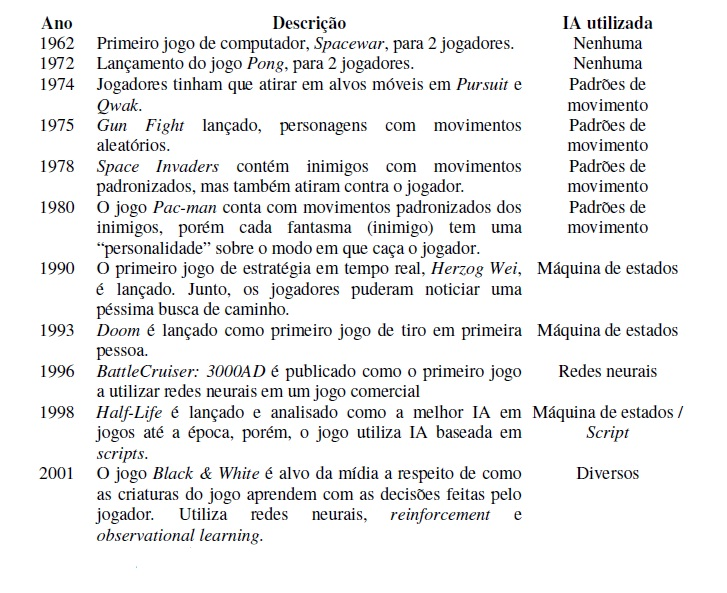
\includegraphics [height=10cm]{figuras/evolucao_IA_jogos.jpg}
\caption{Evolução da aplicação de IA em jogos}
\label{IA em jogos}
\end{figure}



%Um pouco de história, motivação do uso, desafios e problemas comuns.

\subsection{Crença, desejo e intenção --- a arquitetura BDI}

O modelo BDI (\textit{Beliefs Desires Intentions}) foi originalmente proposto por Bratman como uma teoria filosófica do raciocínio prático, propondo uma análise do comportamento humano que seria baseado em crenças, desejos e intenções.
Basicamente supõe-se que as ações são derivadas a partir de um processo chamado raciocínio prático. Este processo é constituído por duas etapas, na primeira, deliberação, o agente seleciona um conjunto de desejos que devem ser alcançados, de acordo com a situação atual das crenças do mesmo. Na segunda etapa ocorre a determinação de como os desejos produzidos no passo anterior podem ser atingidos através do uso dos meios disponíveis ao agente \textbf{[4] Michael Wooldridge, Reasoning about Rational Agents. Cambridge, MA: The M. I. T. Presss 2000.}.
A seguir explicaremos melhor o que são crenças, desejos e intenções.
\begin{itemize}
\item \textbf{Crenças (Beliefs)}: Representam as características do ambiente e são atualizadas constantemente. Podem ser vistas como a componente informativa do sistema.
\item \textbf{Desejos (Desires)}: Representam os objetivos a serem alcançados. Podem ser vistos como motivações do sistema.
\item \textbf{Intenções (Intentions)}: Representam o atual plano de ações escolhido. 
\end{itemize}

A partir deste modelo nasceu a arquitetura BDI para agentes. Agentes BDI são sistemas localizados em um ambiente (em nosso caso o ambiente será virtual) sujeito a variações, além disso, percebem o estado deste ambiente constantemente e podem atuar sobre o mesmo para tentar alterar o estado atual.
Abaixo vemos o processo de raciocínio prático de um agente BDI.
 
\begin{figure}
\centering
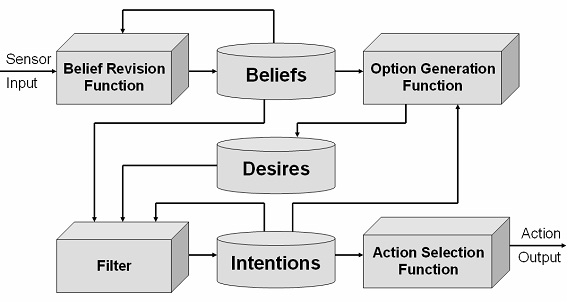
\includegraphics{figuras/visao_BDI.jpg}
\caption{Diagrama de uma arquitetura BDI genérica [4]}
\label{arquitetura BDI}
\end{figure}

Como se pode observar na figura \ref{arquitetura BDI}, existem sete elementos básicos que compõem um agente BDI, são eles \textbf{[5] Ingrid Oliveira de Nunes, Implementação do modelo e da arquitetura BDI}:
\begin{itemize}
\item Um conjunto de crenças (\textit{Desires}) atuais que representam as informações que o agente tem do ambiente.
\item Uma função de revisão de crenças (\textit{Belief Revision Function}), a qual determina um novo conjunto de crenças a partir da percepção da entrada e das crenças do agente.
\item Uma função de geração de opções (\textit{Option Generation Function}), a qual determina as opções disponíveis ao agente (seus desejos), com base nas suas crenças sobre seu ambiente e nas suas intenções.
\item Um conjunto de opções (\textit{desires}) corrente que representa os possíveis planos de ações disponíveis ao agente.
\item Uma função de filtro (\textit{filter}), a qual representa o processo de deliberação do agente, que determina as intenções do agente com base nas suas crenças, desejos e intenções atuais.
\item Um conjunto de intenções (\textit{Intentions}) atual, que representa o foco atual do agente, isto é, aqueles estados que o agente está determinado a alcançar.
\item Uma função de seleção de ação (\textit{Action Selection Function}), a qual determina uma ação a ser executada com base nas suas intenções atuais. 
\end{itemize}

\subsection{Quadro-negro --- blackboard}

	A forma mais simples de apresentar o conceito de blackboard é através de uma metáfora que propõem a seguinte situação \textbf{(Daniel D. Corkill, Blackboard Systems. Blackboard Technology Group, Inc.)}:
 “Imagine um grupo de cientistas reunidos em uma sala trabalhando de forma cooperativa para resolver um problema. Para chegar a uma solução é utilizado um quadro negro (\textit{blackboard}).
A resolução do problema começa quando o mesmo é escrito no quadro negro juntamente com informações iniciais. Os cientistas verificam o conteúdo do quadro e aguardam uma oportunidade para aplicar seus conhecimentos visando solucionar o problema. Quando um cientista encontra informações suficientes para fazer uma contribuição, o mesmo coloca sua contribuição no quadro negro, e com sorte, este processo ativará outro cientista e assim por diante até chegarem à solução do problema.”
	Da metáfora acima se pode concluir que um blackboard possui uma base de dados comum a diversos sistemas que estão tentando solucionar um problema e utilizam e atualizam as informações existentes nesta base de dados.
	 A seguir apresentaremos algumas características desta técnica:
	 \begin{itemize}
	 \item \textbf{Independência de conhecimento}: No exemplo acima, supomos que cada cientista adquiriu seus conhecimentos de maneira independente dos outros, ou seja, num blackboard cada sistema que participa da solução de um problema tem seus próprios níveis de conhecimento, independentemente dos outros sistemas.
	 \item \textbf{Diversidade nas técnicas de solução de problemas}: Uma das grandes vantagens do blackboard é que não interessa como os sistemas que estão trabalhando na resolução do problema funcionam, ou seja, um sistema pode utilizar redes neurais enquanto outro pode utilizar simulações, que para o blackboard estas “fontes de conhecimento” são caixas pretas que fazem suas contribuições.
	 \item \textbf{Representação da informação é flexível}: Não existe nenhuma definição de como deve ser a informação, dando liberdade a quem implementa de definir como representar os dados.
	 \item \textbf{Linguagem comum entre os sistemas}: Ao mesmo tempo em que existe a flexibilidade na representação da informação, é necessário, por outro lado, que todos os sistemas envolvidos sejam capazes de entender tais informações.
	 \item \textbf{Liberdade de organização dos dados}: A organização dos dados é livre, porém, deve ser feita de tal forma que, no caso da base de dados possuir muita informação, seja fácil para um sistema encontrar informações específicas de forma rápida e simples.
	 \item \textbf{Ativações baseadas em eventos}: Os sistemas que estão trabalhando na solução do problema não se comunicam diretamente, ao invés disto, todos “observam” a base de dados comum e utilizando as informações da mesma buscam gerar novos dados que são colocados na mesma base, tais dados podem ativar outro sistema que fará a mesma coisa até que o problema seja completamente resolvido.
	 \item \textbf{Necessidade de controle}: É preciso haver um “órgão” para controlar todos os sistemas e decidir quem deve e quem não deve poder alterar os dados do quadro negro, assim não existe o risco de mais de um sistema alterar uma mesma área de dados simultaneamente.
	 \item \textbf{Geração de solução incremental}: É evidente que a solução de um problema acontece de passo em passo, ou seja, um sistema faz uma contribuição com novos dados, a seguir, outro sistema utiliza tais dados e faz uma nova contribuição e de ciclo em ciclo o problema tende a ser resolvido. 
	 \end{itemize}

Na figura \ref{blackboard} temos uma visão geral de como funciona o blackboard. Basicamente existem fontes de conhecimento (sistemas que estão trabalhando na resolução do problema) um sistema de controle que concede permissões às fontes de conhecimento para alterarem os dados do quadro negro, este por sua vez, é uma base de dados que contem informações que ficam disponíveis a todas as fontes de conhecimento.

\begin{figure}
\centering
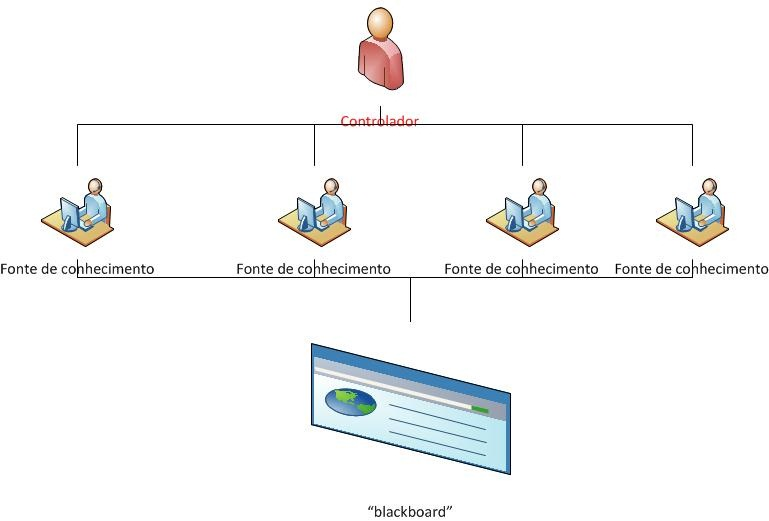
\includegraphics [height=7cm]{figuras/visao_geral_blackboard.jpg}
\caption{Visão geral do blackboard}
\label{blackboard}
\end{figure}
	
Neste projeto utilizaremos a técnica blackboard como parte de um jogo computacional que será desenvolvido.


\subsection{O que avaliar}

\subsubsection{Aspectos humanos} 

Embora o escopo deste trabalho esteja mais próximo de uma avaliação de viabilidade do que de uma análise comparativa de desempenho propriamente dita, vale ressaltar que há espaço, e mesmo a necessidade, de que se estude o impacto da aplicação das técnicas de IA (alvo deste estudo) na experiência de jogo resultante.

Assim, é importante que se tenha em mente que trabalhamos sobre a hipótese de que o campo da inteligência artificial tem a contribuir positivamente na adaptabilidade dos próprios roteiros e trama das histórias que permeiam jogos --- visto que sua aplicação já se dá efetivamente em outros contextos. A expectativa é obter um comportamento mais adaptado ao contexto e enredo em relação que se alcança hoje com máquinas de estado, sem sacrificar o controle que o designer tem.

\subsubsection{Aspectos técnicos e de projeto}

Existe um aumento na complexidade dos diálogos, em razão da necessidade de incorporar mais informações de contexto e variantes no jogo. Isso se traduz na composição de um número maior de derivações em diálogos, já que tanto o jogador quanto os \npc{}s passam a ter opções, e também a necessidade de projeto dos agentes em si.

\subsubsection{Aspectos gerais}

É interessante que se avalie o processo de adaptação das técnicas empregadas ao estudo feito, e se elas podem ser aplicadas a outros domínios. Em particular, o que jogos de diferentes gêneros podem ganhar com o uso da engenharia de software voltada a agentes e de técnicas como por exemplo, blackboard.
%O que o estudo de caso vai avaliar, e como. Decisões de projeto que
%validam o estudo (C++, \emph{data-driven} design, prototipação,
%engenharia de software), isto é, porque o projeto permite extrapolar
%conclusões para jogos na indústria.

\chapter{Especificação}

%Nesta seção descrevemos os critérios de aceitação do projeto:
%\begin{itemize}
%\item descrição das telas,
%\item opções esperadas dos menus,
%\item comportamento esperado dos \npc{}s
%\end{itemize}

Neste capítulo abordam-se os requisitos que o projeto deve satisfazer para que o estudo de caso seja efetivo. Foi dada atenção particular à aderência do projeto a padrões industriais de metodologia de desenvolvimento de jogos, na medida em que tal não se mostrasse incompatível com o escopo de um projeto de formatura. 

Assim optou-se pelo emprego do GDD (Game Design Document --- apêndice~\ref{ap:gdd}) como meio de especificação e captura de requisitos do projeto. Da mesma forma foram tomadas decisões como a escolha das linguagens e bibliotecas empregadas, tendo em vista padrões recorrentes na indústria e portabilidade.

\section{Decisões de projeto}

\subsection{Limitações e controle da expressão dos agentes}

Apesar de variabilidade e adaptabilidade da experiência do jogo
constituírem, em grande medida, o que se busca ao introduzir-se algum
modelo de inteligência na lógica de jogos, é preciso ter em mente que
isso não significa que se queira abrir mão do design dessa
experiência. De fato, parte da complexidade da incorporação de
inteligência artificial a jogos advém da necessidade de identificar
que aspectos da dinâmica da inteligência devem ser coergidos, moldados
ou mesmo eliminados, em prol de atributos como a jogabilidade e mesmo
adaptação às limitações e anseios dos jogadores.

Nesse sentido, optou-se por um modelo --- experimental e
por vezes potencialmente limitante, como será visto adiante ---
restritivo de expressão dos agentes que controlam o diálogo com
\npc{}s.

O modelo implementado tem por ideia central que os diálogos são
interações de \emph{estímulo e reação} do agente inteligente pelo
jogador. Os estímulos estão associados ao que o jogador opta por
dizer, e as reações às opções de fala do \npc. 

As opções de um e outro estão registradas nos \emph{roteiros de
  diálogo}, que são compostos pelos designers do jogo. Nesses
roteiros, as falas de jogador e agente estão descritas, e tanto os
estímulos que transmitem quanto as reações que expressam são definidos
por uma \emph{marcação de conteúdo}. Assim, uma saudação pode ser um
estímulo amigável; uma afirmação pode soar suspeita; e, por outro
lado, uma interjeição pode expressar contentamento ou rabugice.

Desse modo, o conjunto de condições passíveis de
expressão pelos agentes fica sob controle do designer do jogo, por
causa da estreita ligação entre os diálogos e os estímulos e
manifestações disponíveis para os agentes. Essa é uma característica
extremamente desejável, como já foi dito, por permitir introduzir a
variabilidade de maneira controlada e em sintonia com a experiência
que se quer produzir.

Existem algumas dificuldades inerentes a esse processo de
modelagem. Está sujeito a avaliação se em projetos de maior porte a
tarefa de gerência dos vários estímulos e reações não se tornaria
proibitiva do uso da técnica.

\subsection{Licença e implicações}

Desde o princípio fez-se a opção por desenvolver um projeto que se adaptasse à filosofia dos softwares livres, de código aberto. Essa característica teve consequências importantes e decisivas no encaminhamento do projeto durante toda a sua evolução. 

Apesar da severidade que as restrições impostas por uma licensa livre ao projeto, deve-se frisar que essa escolha se apresentou certa para o grupo. Não só é inegável o caráter inerentemente livre da produção acadêmica de universidades públicas, meio em que se insere este projeto, como é preciso que se diga que há uma janela de oportunidade na atual carência, no universo dos softwares livres, de projetos de jogos. Essa carência, note-se, vem sendo paulatinamente alvo de estudos e experimentações no mercado, fato que se observa pela progressão do número de títulos que vêm sendo portados para sistemas livres.

Há duas consequências de grande impacto prático na condução do projeto de um jogo livre,  a saber a restrição no uso de software de terceiros e de conteúdo midiático que pode ser aproveitado. Como será discutido adiante (seção~\ref{sec:tradeoffs}), essa opção reduziu a gama de arcabouços de tecnologia que puderam ser aproveitados, e impôs ao projeto a responsabilidade pela criação de parte da arte do jogo --- uma carga de trabalho não desprezível dado escopo e recursos disponíveis.  

\subsection{Tecnologias empregadas}\label{tecnologias_empregadas}

Uma das primeiras decisões que foram tomadas na definição das condições de contorno do projeto foi que a linguagem empregada para desenvolvimento do software deveria refletir algum padrão solidamente estabelecido na indústria. Optou-se por C++, uma linguagem que goza de grande popularidade na idústria com títulos conhecidos como \emph{Doom} e \emph{Age of Empires}.

Outra decisão de impacto foi a escolha de engines. À partir de uma primeira lista, compilada por meio de pesquisas em fóruns de discussão sobre desenvolvimento de jogos, construiu-se uma matriz de decisão em que foram eliminadas as opções que não apresentavam licensas livres, portáveis e que não possuíssem interface com C++. Por fim escolheu-se empregar o Simple DirectMedia Layer (SDL), linguagem de interface portável com dispositivos de media e periféricos\footnote{Como um adendo, citamos dois títulos conhecidos que usam SDL em pelo menos uma versão: \emph{World of Goo} e \emph{Doom 3}.}.

O uso da ferramenta Jason, para a criação dos agentes, se deve principalmente ao fato de que o projeto nasceu motivado pela tese de doutorado~\cite{tese_roberto} de um dos orientadores do grupo que, no desenvolvimento de seu projeto, utilizou a ferramenta. Além disso, como esta ferramenta é baseada em Java, parte do projeto foi desenvolvida utilizando essa linguagem.

%Escolhemos C++ porque é bastante usado na indústria.
%Fizemos uma matriz de decisão cruzando informações sobre diversos engines de %renderização, e baseamos a decisão segundo as restrições: tem que ser livre, tem que ser %portável, tem que dar pra usar com C++.
%Jason -> ferramenta “bonitinha” para se trabalhar com sistemas de agentes inteligentes.
%-> SDL, Jason (plug-in para eclipse), C++.


\section{Especificação dos requisitos do software}
Conforme o modelo de desenvolvimento adotado pela indústria, os requisitos do software foram levantados a partir do GDD e das decisões de projeto. Vale ressaltar que no caso do desenvolvimento de jogos, o documento de consulta primário é o GDD.

É importante citar que a grande maioria dos requisitos funcionais do software são regras do jogo e estão descritos no documento de game design. Dentre os outros requisitos funcionais temos:
\begin{itemize}
\item O software deve fazer e administrar a comunicação entre os módulos implementados em C++ e Java.
\item O diálogo entre o usuário e um \npc{} não pode parecer determinístico.
\end{itemize}

Os requisitos não-funcionais levantados foram os seguintes:
\begin{itemize}
\item A comunicação entre os módulos implementados em Java e C++ não deve demorar mais que 3 segundos.
\item As tecnologias envolvidas no projeto devem ser livres.
\item A interface homem-máquina deve ser simples e intuitiva
\item O tempo de processamento de dados no blackboard não pode ser superior a 5 segundos.
\end{itemize}

\chapter{Metodologia}

O sucesso de um projeto depende em grande medida da capacidade de
adaptação dos envolvidos. Nesta seção tratamos do método de
planejamento de atividades do trabalho, e de sua evolução no decorrer
do projeto. Assim, em certa medida trataremos das mudanças que se
operaram nas expectativas e previsões que fizemos ao longo do tempo.

\section{Evolução}

Nesta seção discorre-se brevemente sobre as atividades desenvolvidas durante o projeto, desde sua especificação às etapas finais de sua implementação.

A ideia de desenvolvimento de um projeto no campo de jogos nasceu há mais de um ano, e diversos assuntos foram elencados como possíveis temas para o projeto de conclusão de curso. Mas foi somente em março de 2010 que a equipe se consolidou e o professor doutor Ricardo Nakamura aceitou orientar o grupo, dando início ao processo de refinamento do tema do trabalho. Foi então que entramos em contato com o professor doutor Roberto Cezar Bianchini, co-orientador do projeto, e autor da tese de doutoramento~\cite{tese_roberto} que sugeriu o tema do presente estudo de caso.  

As primeiras atividades do grupo então concentraram-se na elaboração de um primeiro cronograma, e foram selecionados assuntos a pesquisar. Nesse ponto foi iniciada a composição de um diário de bordo, em que se registrou todo o avanço do projeto.

O passo seguinte foi solidificar as condições de contorno do problema, por meio de reuniões em que se procurou unificar a visão dos envolvidos, progredindo gradualmente rumo a uma concepção amadurecida dos objetivos e métodos a serem empregados no projeto.

Após diversas reuniões, o grupo optou por utilizar uma linguagem de presença expressiva na idústria: C++ (conforme justificado na seção~\ref{tecnologias_empregadas}); além disso, estipulou-se que o projeto teria uma licença livre.

Com relação ao jogo, o grupo optou por desenvolver um jogo em 2D, esta escolha foi feita para simplificar o desenvolvimento, uma vez que a parte gráfica do jogo não era o foco do projeto.
O grupo procurou simuladores de sistemas multi-agentes que trabalhassem com a arquitetura BDI. Por fim, o grupo buscou listar os requisitos de engines e softwares de renderização que viria a utilizar.

O grupo então definiu que a parte gráfica do jogo seria implementada usando SDL. Além disso, o grupo decidiu trabalhar com a ferrametna Jason para o desenvolvimento de sistemas multi-agentes, fato que implicou diretamente na escolha da linguagem Java como auxiliar no desenvolvimento do projeto.
Após esta decisão, nasceu a necessidade de se criar uma forma de comunicação entre as partes do jogo que foram desenvolvidas em Java e em C++, a solução escolhida foi fazer comunicação usando TCP via loop-back (foram analisadas outras soluções, porém nenhuma delas eram tão simples quanto a solução adotada). Após esta etapa a arquitetura do software começou a ficar mais transparente aos envolvidos, isto foi importante pois permitiu que o trabalho fosse dividido de forma eficiente entre o integrantes do grupo.

A seguir, o grupo apresentou aos orientadores uma proposta de um jogo que já envolvia os conceitos que foram abordados no projeto. Após algums reuniões sobre a proposta surgiram os primeiros rascunhos do documento de design do jogo.

Com a consolidação da proposta, o grupo efetuou uma primeira divisão de responsabilidades de estudos, particionando os assuntos em escopos de conhecimento: tecnológico (C++, BDI, Java, AgentSpeak, SDL, e arquiteturas de software empregadas em jogos).
Ficou definido que toda a lógica do jogo e a parte gráfica seriam implementadas em C++, enquanto os agentes e o blackboard seriam desenvolvidos em AgentSpeak e Java respectivamente.

Esse estudo acompanhou o desenvolvimento do projeto até estágios avaçados, mas após alguns meses desde seu início preparou-se um cronograma mais detalhado, adiantado propositadamente de modo que as atividades previstas se encerrassem com um mês de antecedência em relação às datas oficiais de entregas e apresentações do projeto, de modo a acomodar sem transtornos eventuais imprevistos --- que, adianta-se, ocorreram.

Esse cronograma destacava as atividades que então foram consideradas essenciais
\begin{itemize}
\item Formação da equipe
\item Escolha do orientador
\item Testes com as tecnologias
\item Escolha das tecnologias
\item Estudo das tecnologias
\item Integração das tecnologias
\item Game Design
\item Especificação dos requisitos
\item Protótipo do software
\item Testes do protótipo
\item Validação
\end{itemize}

A composição do GDD iniciou em fins de abril, baseando-se em previas e estudos de conceito do jogo que haviam sido armazenados no decorrer do semestre, e estendeu-se até meados de agosto. Este segundo cronograma estimava já o tempo de implementação dos componentes da arquitetura do sistema --- como era concebido então --- além de estimar o tempo que a equipe levaria para encontrar conteúdo artístico com licensa compatível com a do projeto e, paralelamente, modelar os agentes do sistema.

Já no segundo semestre o grupo reestruturou o cronograma criando pontos de avaliação do progresso do desenvolvimento (\emph{milestones}), quando então ocorriam encontros com os orientadores em que se apresentava o progresso, comparavam-se as metas previstas e alcançadas, faziam-se novas estimativas para conclusão do que não se havia cumprido, e discutiam-se os problemas encontrados e vislumbrados para o futuro. As milestones estão listadas abaixo. Outras alterações de impacto na visão da equipe sobre as etapas por futuras do projeto foi o acerto de uma divisão de tarefas mais acirrada nas etapas finais, concentrando-se um e outro em áreas que bem conheciam. Desse modo, Murilo ficou responsável pela parcela do projecto associada à inteligêngia e modelagem de agentes, enquanto Tássio trabalhou com a lógica e renderização do jogo. A elaboração do protocolo de comunicação entre os agentes e a lógica do jogo foi feita em conjunto, assim como a elaboração dos diálogos.

\subsection{Primeira milestone (30 setembro)}
\begin{itemize}
\item pesquisa de coleções de arte (gráficos e som) que serão usadas no trabalho
\item porte do projeto para o Subversion
\item solução para comunicação entre processos Java e C++ do jogo
\item elaboração de tabelas para modelagem de características de personagens do jogo.
\item mecanismos de escrita e leitura do quadro-negro (blackboard)
\item roteiro de aceitação do projeto
\item capítulos introdutórios e de especificação da monografia
\end{itemize}

Das atividades listadas na primeira milestone, apenas os mecanismos de escrita e leitura no blackboard e o roteiro de aceitação do projeto não respeitaram a data proposta. Isso se deveu ao fato de que ainda havia a necessidade de aumentar o nível de detalhamento  nas especificações do jogo e da arquitetura do software como um todo. Por outro lado, o grupo foi capaz de adiantar algumas atividades definidas nas outras milestones, tais como a modelagem de agentes mais simples e subsistemas da lógica do jogo.

\subsection{Segunda milestone (15 outubro)}
\begin{itemize}
\item navegação pelos modos e telas do jogo funcional
\item quadro-negro (blackboard) com um tipo de conhecimento compartilhado
\item modelagem de alguns agentes mais simples
\item módulos de menus e diálogos
\item capítulos de sobre decisões de projeto da monografia
\end{itemize}

Por essa data o projeto já contava com testes funcionais de controle de todos os subsistemas que o jogo precisaria, e já havia sido alcançada a integração entre áudio e vídeo, documentada em pequenos demos (tópico da terceira milestone). Nesse ponto, a equipe já tomou consciência de que a complexidade de alguns tópicos havia sido superestimada, enquanto a de outros subestimada. O grupo cogitava então participar do IX Simpósio Brasileiro de Games (SBGames).

\subsection{Terceira milestone (25 outubro)}
\begin{itemize}
\item integração de áudio e gráficos
\item terminada modelagem de todos os agentes do jogo
\item quadro-negro compartilhando conhecimento de classes diversas
\item testes de integração do sistema
\item capítulos sobre projeto dos testes, resultados e conclusões da monografia
\end{itemize}

À terceira milestone o projeto havia atingido um estágio delicado. Boa parte do conhecimento necessário para sua conclusão já estava cominado pela equipe, mas algumas decisões importantes para a estruturação do e funcionamento do projeto estavam pendentes, necessitando de ajustes. O grupo por esta época já havia decidito participar do SBGames, como ouvinte (a princípio havia-se cogitado expor um artigo curto sobre o trabalho de conclusão de curso no evento).   

\subsection{Quarta milestone (5 novembro)}
\begin{itemize}
\item monografia completa
\item elaboração de roteiro de apresentação e material (capturas de tela, videos, etc.)
\end{itemize}

Infelizmente um dos integrantes teve que cancelar sua ida ao SBGames de última hora, em razão de seu estágio. De todo modo, a apresentação de milestones ficou suspensa durante uma semana --- mesmo porque um de nossos orientadores estava participando do simpósio.

\subsection{Percalços e reajustes}

Um fato que prejudicou o andamento do projeto foi que ambos os integrantes do grupo começaram a estagiar. Inicialmente este fato não parecia influenciar no desempenho dos integrantes, no entanto, conforme os estágios começaram a exigir mais tempo e dedicação o andamento do desenvolvimento diminuiu.
Uma parte do desenvolvimento que realmente surpreendeu o grupo foi a criação dos diálogos. O grupo sempre acreditou que a criação dos arquivos de diálogos seria uma atividade demorada, no entanto, esta atividade foi muito mais complexa do que esperado, isso se deve ao fato de que cada arquivo de diálogo deve conter opções de falas tanto para o jogador quanto para os \npc{}s, sendo assim, cada diálogo do jogo, por mais simples que fosse, virou um arquivo de texto muito extenso.
Um fato que atrasou um pouco o desenvolvimento do jogo foi a falta de conhecimento sobre os temas, os alunos ainda não tinham nem um contato com os conceitos de IA nem sobre programação orientada a agentes. Foram necessárias horas de estudos sobre os assuntos antes dos integrantes do grupo conseguirem iniciar o desenvolvimento.


\subsection{Considerações sobre aplicação da metodologia}

É a percepção do grupo que houve uma adaptação das esperanças e estratégias de mobilização, planejamento, discussão e trabalho à medida que o projeto amadureceu, e adiquiriu-se maior confiança do que se poderia alcançar. Calibramos, aos poucos, a medida da incerteza de nossas previsões, e, embora seja inegável que há muito o que aprimorar, vislumbrou-se evolução considerável na habilidade de cada membro da equipe de lidar com imprevistos e incertezas, o que se mostrou crucial para que o término exitoso do projeto fosse alcançado.

É importante destacar o papel que a aquisição de conhecimento no domínio do projeto --- e com isso referimo-nos tanto ao estudo técnico quanto ao conhecimento adquirido pelo contato com pessoas do ramo --- na mudança da própria maneira e enfoque do projetar e compreender o projeto do jogo. Nesse contexto é notável o papel que desempenhou o curso da disciplina Design e Programação de Games no segundo semestre de 2010, assim como a participação no SBGames, nos quais adiquiriu-se um conhecimento que, de certo modo, não está acessível por meio das vias consagradas de estudo; um conhecimento vivo, orgânico, da esfera cultural que é parte inerente dos jogos neste tempo.



\chapter{Implementação}

Neste capítulo descrevemos brevemente o sistema, abordando a organização de seus arquivos componentes e a estratégia de organização do software tendo em vista a criação de uma estrutura de fácil manutenção e expansão.

\section{Visão global}

O jogo é disparado por um pequeno aplicativo cuja única função é iniciar\footnote{Isso foi feito por meio do fork to processo e alteração de suas imagens nos processos pai e filho resultantes.} os componentes Java e C++ do projeto, que passam então a se comunicar via TCP (via \emph{loopback}), empregando a porta de número especificado no arquivo de configuração.

Passada essa etapa de estabelecimento de comunicação, a interação entre C++ e Java se dá pela troca de mensagens, segundo um protocolo simples desenvolvido no trabalho para este projeto em particular. Sua descrição consta no apêndice~\ref{ap:protocolo}. As responsabilidades ficam então assim divididas: a renderização e gerenciamento dos arquivos de diálogos e variáveis do jogo (inventário, membros ativos da gangue, recursos financeiros, etc.) fica a encargo do programa C++, enquanto que toda a tarefa de simulação da arquitetura  BDI e da gerência do blackboard, assim como manutenção do registro dos estados psicológicos, personalidade e conduta dos agentes são de responsabilidade do programa Java (o que inclui o interpretador de AgentSpeak, Jason). Ademais, na arquitetura implementada, o processo Java roda como cliente TCP, e o C++ como servidor.

%Como as coisas funcionam. O que faz o quê (macroscopicamente).

%Uma explicação sucinta da estrutura do programa, como ele inicia
%(forking) e como age em regime (responsabilidades java vs C++, e o
%protocolo).

\section{Compromissos (\emph{trade-offs})}\label{sec:tradeoffs}

Esta seção descreve algumas opções que o grupo fez, sacrificando certos atributos desejáveis em prol de outros no projeto. 

Já foi mencionado que a opção por uma licensa livre para o projeto incorreu tanto em beneífios como em perdas para o projeto. Passou-se a dispor de espaço para hospedagem do projeto, por um lado, embora, por outro, tenha sido necessário abrir mão do uso de engines e bibliotecas proprietárias para o desenvolvimento.

Outro ponto de compromisso foi a decisão por um modelo ``fechado'' de respostas de agentes nos diálogos: a reação dos agentes nesse caso ficou restrita ao conjunto de opções previstas pelo escritor do diálogo. Se por um lado perde-se com a restrição da manifestação do BDI a um conjunto pré-modelado de respostas, por outro ganha-se em condução do diálogo, uma vantagem que não pode ser menosprezada no design do jogo.

Um ponto de destaque foi a decisão de trabalhar com mais de uma linguagem de programação, o fato de trabalharmos com C++, Java e AgentSpeak gerou a necessidade de se desenvolver protocolos de comunicação para integrar os subsistemas, fato este que consumiu bastante tempo e dedicação do grupo.

Por fim, devemos mencionar que, dado o escopo temporal do projeto, optamos por simplificações na sofisticação da renderização. O ganho de tempo dedicado ao projeto veio, nesse caso, às custas de um distanciamento do objeto-alvo de estudo, jogos comerciais, uma vez que o investimento n desenvolvimento de uma apresentação gráfica adequada é uma preocupação constante nesse meio.

\section{Arquitetura}

Conforme descrito anteriormente, a arquitetura do sistema é baseada em dois grandes subsistemas. O subsistema implementado em Java que inclui os códigos interpretados pelo Jason e o subsistema implementado em C++. A figura \ref{arquiteturaGeral} ilustra esta situação.

\begin{figure}
\centering
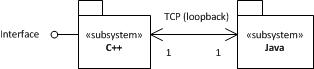
\includegraphics{figuras/arquitetura.jpg}
\caption{Visão geral da arquitetura do sistema}
\label{arquiteturaGeral}
\end{figure}


\subsection{Subsistema: Java}

A figura \ref{arquiteturaJava} apresenta a arquitetura do subsistema implementado em Java. Existem três classes principais, \emph{Manipuladora}, \emph{Comunicadora} e \emph{Level}.
A classe Manipuladora é responsável por consultar e manter atualizados os arquivos de modelos de agentes (explicados em \ref{estruturaPastas}), já a classe Comunicadora é a responsável por receber, enviar e traduzi as mensagens que chegam através da conexão com o subsitema C++. Ambas as classes se comunicam com a classe Level que nada mais é do que a classe de ambiente dos agentes. A classe Level é uma classe utilizada pelo Jason, ela representa o ambiente (enviroment) e é nela que todas as ações dos agentes foram implementadas, no caso deste programa as ações dos agentes são basicamente escolher um tipo de resposta ou atualizar variáveis de controle dos agentes e dos lugares.

\begin{figure}
\centering
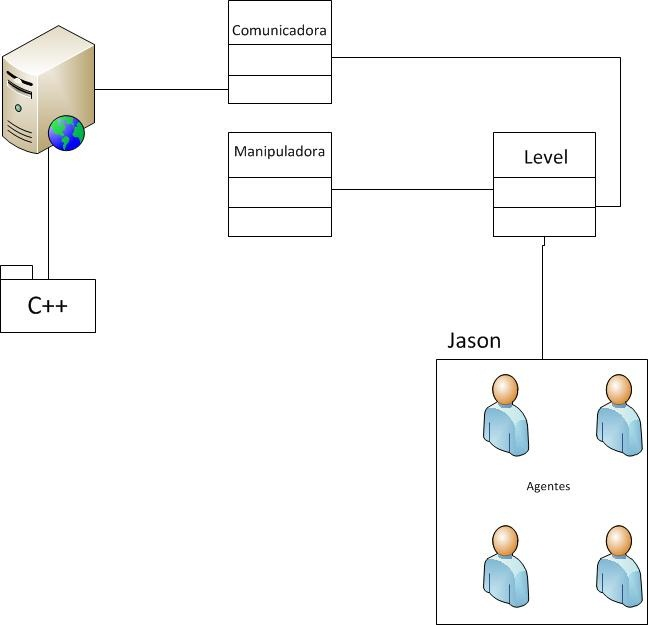
\includegraphics[height=10cm]{figuras/arquitetura-java.jpg}
\caption{Visão geral da arquitetura do subsistema Java}
\label{arquiteturaJava}
\end{figure}

\subsubsection{Arquitetura BDI}
Após pesquisas, o grupo encontrou um \emph{plug-in} do interpretador Jason para rodar com a IDE eclipse, com isto o trabalho ficou mais simples, todo a parte do projeto que utilizava linguagem Java e AgentSpeak foi implementada utilizando a IDE eclipse.
A arquitetura dos agentes não ficou complexa, basicamente todos possuem caracterísicas em comum como a \emph{personalidade} e o \emph{estado psicológico}. No caso de um diálogo estas duas características são necessárias pois é baseado nelas que o agente toma decisões, a atualização destas características ocorre da seguinte forma:
\begin{enumerate} 
\item Classe comunicadora recebe mensagem do tipo estimuloagente ( num agente, num estímulo )
\item Classe Level recebe os parâmetros e insere a crença estímulo(nomeEstimulo) no agente em questão
\item Agente atualiza sua personalidade e seu estado psicológico
\end{enumerate}

Caso o agente receba opções de resposta, ele avalia o(s) estímulo(s) recebido pela fala do jogador e procura a resposta que contenha a reação que lhe interessa, este processo acontece da seguinte forma:

\begin{enumerate} 
\item Classe comunicadora recebe mensagem do tipo estimuloagente ( num agente, num estímulo )
\item Classe Level recebe os parâmetros e insere a crença estímulo(nomeEstimulo) no agente em questão
\item Agente atualiza sua personalidade e seu estado psicológico
\item Classe comunicadora recebe mensagem do tipo ofereceEscolhas( num agente, num reacao1, num reacao2, ... )
\item Classe Level recebe os parâmetros e insere a crença respostas(reacao1,reacao2) no agente em questão
\item O agente procura em sua lógica qual a melhor reacao segundo sua personalidade e seu estado psicológico 
\item O agente executa a ação responder(reacao) que envia para o subsitema C++ a escolha do agente
\end{enumerate}

Os casos demonstrados acima se aplicam a qualquer agente com o qual o jogador inicie um diálogo, inclusive os capangas, isto foi feito para manter a arquitetura dos agentes mais genérica.

\subsubsection{Blackboard}

A técnica \emph{blackboard} foi implementada dentro da arquitetura dos agentes ocultos da polícia, esta decisão de projeto visou um melhor desempenho do software.
Basicamente foi criado um agente oculto para cada tipo de informação que pode ser enviada por um agente policial, assim, toda vez que um agente policial executar a ação \emph{avisaPolicia(sujeito,predicado)} é adicionada uma crença em cada agente oculto sobre este aviso, no entanto, apenas um deles sabe o que deve fazer com esta informação, este agente processa a informação e avisa todos os outros agentes a nova informação, esta nova informação pode ser uma ação da polícia que será enviada aos agentes policiais ou pode ser uma nova informação que outro agente oculto sabe processar, assim o processo se torna incremental até que a informação seja completamente processada e resulte em algum tipo de ação da polícia.


\subsection{Subsistema: C++}

A concepção do subsistema C++ foi talvez uma das etapas mais longas do
projeto. Isto pois exite toda uma série de questões inerentes à a organização
do controle da lógica e renderização de jogos, e, como é natural em
sistemas complexos, pequenas decisões da estrutura e organização
refletem grandemente na adequação do sistema à manutenção e
alterações.

Manteve-se em mente durante o pojeto que, dada a novidade do campo de
desenvolvimento de jogos para os integrantes do grupo, dever-se-ia
optar por soluções mais afeitas à modificações. Essa opção é natural,
dado que era grande a probabilidade de que fosse neessário efetuar
modificações para comportar necessidades identificadas ao longo do
desenvolvimento. Ademais, a metodologia de design do jogo escolhida
valia-se de prototipações frequentes, e, nesse sentido, foi importante
que o sistema em si refletisse essa flexibilidade, de modo a atender
às requisições de alteração de comportamento exigidas pela
experimentação com a lógica do jogo. Ressaltamos, entretanto, que essa
flexibilidade não foi total, e desde muito cedo o projeto se fixou em
restrições de apresentação gráfica, numa tentativa de se guardar certo
controle sobre o crescimento da complexidade da renderização do jogo.

Posto de maneira simples, o jogador transita no jogo por estados, como
o \emph{menu principal}\footnote{Menu que permite optar por iniciar um
  novo jogo, carregar um jogo salvo, ou terminar o aplicativo.}, o
\emph{mapa da cidade}\footnote{Mapa por meio do qual o jogador obtém
  acesso à ações como roubar um estabelecimento, fazer compras no
  mercado, etc. (vide o documento de game design, na
  seção~\ref{fluxo-jogo}).}, \emph{diálogos} e \emph{cenas}, 
\emph{gerência de seu inventário de itens}, \emph{compra no mercado} e
\emph{planejamento do roubo}\footnote{Sequência de telas que
  compreende a seleção de participantes do roubo, equipamento a usar,
  e disribuição das recompensas.}. Cada estado é uma abstração de um
conjunto de interações que o jogador pode ter com o jogo.

Foram encapsuladas as primitivas da biblioteca SDL em classes que
\emph{gestoras de recursos}. Esses recursos são
\begin{itemize}
\item imagens (carregadas para serem exibidas na tela,
\item sons,
\item fontes, e
\item eventos.
\end{itemize}

A conexão com o subsistema Java também foi feita encapsulando-se uma
interface SDL, e adaptou-se o sistema interno de captação e
comunicação de eventos do SDL para incorporar as mensagens do
protocolo de comunicação elaborado (vide apêndice~\ref{ap:protocolo}).

Outras abstrações implementadas incluem \emph{design-patterns} como
\emph{decoration}, \emph{strawman}, \emph{singleton}, \emph{factory} e
\emph{interface}. Por exemplo, objetos que queiram ser informados de
eventos do protocolo devem ser \emph{EventListeners} e se inscrever na
lista de ouvintes do \emph{EventManager}, servidor de mensagens do
jogo. Analogamente, objetos que queiram ser desenhados devem ser
\emph{Drawable} e se inscreverem (ou serem inscritos) em alguma
\emph{View} (objetos gerenciadores de exibição de imagens na
tela).

Finalmente, mas não menos importante, o laço principal do jogo
constitui-se da constante medida do tempo decorrido (em milisegundos)
desde a última execução do laço. Este valor é passado para um método
de atualização do gerenciador de estados
(\emph{StateManager}\footnote{Os estados são objetos em uma pilha,
  gerenciada pelo \emph{StateManager}. Ele também é o responsável pela
criação e destruição dos estados.}), que faz o controle da taxa
de atualização da tela.




\section{Protocolo de comunicação}

A necessidade de comunicação entre os subsistemas de processamento da inteligência articial implementada e os mecanismos de controle e renderização do jogo surgiram tão logo se foram definidos dois requisitos do projeto, em seu início: o emprego de C++, de modo a refletir um padrão amplamente empregado na indústria de jogos, e a opção pelo uso do interpretador de AgentSpeak, Jason, que possui apenas interfaces para Java.

Definiu-se então um protocolo simples, operando via TCP (\emph{loopback}), o que não incorre em perdas significativas de eficiência na troca de informações. O protocolo, que passou por diversas modificações ao longo da evolução do projeto, baseia-se na troca de mensagens, sequencias de inteiros, que respeitam regras simples:
\begin{enumerate}
\item o primeiro inteiro enviado representa quantos inteiros mais compõe a mensagem;
\item o segundo inteiro identifica o nome da mensagem;
\item os demais inteiros são parâmetros da mensagem.
\end{enumerate}

O nome da mensagem é recuperado pelo receptor da mensagem pela leitura de um arquivo de referência --- é a linha de número igual ao inteiro recebido. Munido dessa cadeia de caracteres, o receptor então pode buscar em um mapa interno a função responsável por tratar a mensagem e seus argumentos. De modo análogo, os argumentos representam, na maior parte das vezes, o número da linha que deve ser lida em algum arquivo do sistema (pré-definido para cada nome de mensagem) contendo algum complemento da informação.

\subsection{Arquivos consultados}

Os arquivos que são lidos pelas rotinas de tratamento das mensagens são
\begin{description}
\item[estímulos] contém estímulos que podem ser enviados a agentes no decorrer de diálogos;
\item[respostas] contém as respostas que agentes podem expressar em diálogos;
\item[capangas] contém nome (e possivelmente outras informações) a respeito de capangas na equipe dos \nomeGrupo;
\item[lugares] contém o nome de lugares passíveis de roubo;
\item[predicados] contém uma lista de avisos que podem ser dados à polícia;
\item[configurações] contém, respectivamente, em suas linhas
\begin{enumerate}
\item o número da porta de comunicação loopback empregado pelos subsistemas em sua comunicação;
\item o número de slots que o jogo possui
\item o maior nível de suspeita possível para capangas (que é também o maior nível de segurança para lugares)
\end{enumerate}
\end{description}

\subsection{As mensagens}

O conjunto de mensagens passou por várias alterações desde sua primeira concepção, o que não somente era esperado, como demonstrou a utilidade da arquitetura de troca de mensagens que havia sido projetada, preparada para acomodar sem grande dificuldade adições e remoções de mensagens. As mensagens são listadas a seguir.

\begin{enumerate}\footnotesize
\item \verb!iniciaDialogo( )! solicita o envio do id de um agente com
  quem o jogador está iniciando um diálogo (o perfil e estado
  psicológico do agente são sorteados pelo subsistema Java);
\item \verb!retornaIdAgente()! retorna um id solicitado por \verb!iniciaDialogo()!;
%
\item \verb!estimuloagente ( # agente, # estímulo )! estimula o agente
  referido;
%\item \verb!atualizaBeliefs(# agente, # estimulo)! 
%
\item \verb!ofereceEscolhas( # agente, # reacao1, # reacao2, … )!
 lista uma série de reações que o agente pode expressar;
\item \verb!returnEscolha(# agente, #escolha)! retorna a escolha
  escolhida pelo agente como a que mais se aproxima de expressar seu
  estado psicológico atual;
%
%
\item \verb!fimDialogo( #agente )! avisa o término do diálogo;
\item \verb!acaoDaPolicia( #acao, #alvo )! solicita ao jogo que tome
  alguma ação em nome da polícia; ações previstas incluem
  \begin{itemize} 
  \item  aumentar nivel suspeita de capanga (alvo);
  \item  diminuir nivel suspeita de capanga (alvo);
  \item  prender  capanga (alvo);
  \item  aumentar nivel segurança de lugar (alvo);
  \item  diminuir nivel segurança de lugar (alvo);
  \end{itemize}
%
\item \verb!avisaPolicia( #sujeito, #predicado )! informa a polícia de
  algo:
  \begin{itemize}
  \item alguém fez compra suspeita;
    \item tentativa de roubo (sucesso);
      \item tentativa de roubo (sucesso);
  \end{itemize}
\item \verb!avisaPolicia( #sujeito, #predicado, #alvo )! informa a
  polícia de algo sobre alguém;
  \begin{itemize}
  \item alguém agiu de modo suspeito em um dado lugar;
  \end{itemize}
%[10 escreveBlackBoard(#sujeito, #predicado)] => 8
%
\item \verb!loadGame(! \#slot \verb!)! solicita carga de jogo;
\item \verb!newGame(! \#slot \verb!)! solicita novo jogo;
\item \verb!saveGame(! \#slot \verb!)! sollicita salvamento de jogo
\item \verb!quitGame()! informa fim de jogo.
\end{enumerate}

A concepção do protocolo de comunicação envolveu alguns cuidados especiais, e precauções foram tomadas no sentido de preservar a flexibilidade do protocolo --- isto é, facilitar a adição de novas mensagens no decorrer do projeto --- e garantir certo desacoplamento entre o trabalho de modelagem de agentes e projeto do blackboard, de um lado, e a lógica do jogo, de outro. Buscou-se organizar a comunicação entre Java e C++ de modo tal que o projeto pudesse ser levado a cabo sem a necessidade de programadores de um e outro sistema precisassem saber do funcionamento do outro. Essa flexibilidade permite que as responsabilidades dos sistemas sejam alteradas durante a evolução do projeto, o que é importante para permitir a exploração de possibilidades de organização do jogo como um todo. Para isso, é necessário que os protótipos construídos não enfrentem as restrições de uma arquitetura rígida.

\section{Estrutura de pastas}\label{estruturaPastas}

O projeto foi desenvolvido com vistas a se prestar à experimentação no
design. Assim, algumas ferramentas para a escrita de \emph{scripts} de
diálogos ou pequenas cenas foram desenvolvidas.

Descrevemos a seguir a organização dos arquivos do projeto. É
importante que essa estrutura seja clara e intuitiva, já que é nossa
intenção que alguns desses arquivos (que configuram o comportamento
do jogo) sejam alterados primariamente por designers do jogo. Assim, é
preciso que haja critério na complexidade que se expõe a esses
``usuários''. A figura~\ref{fig:estrut-arquiv} exibe a distribuição de arquivos nas pastas do projeto.  

\begin{figure}
\centering
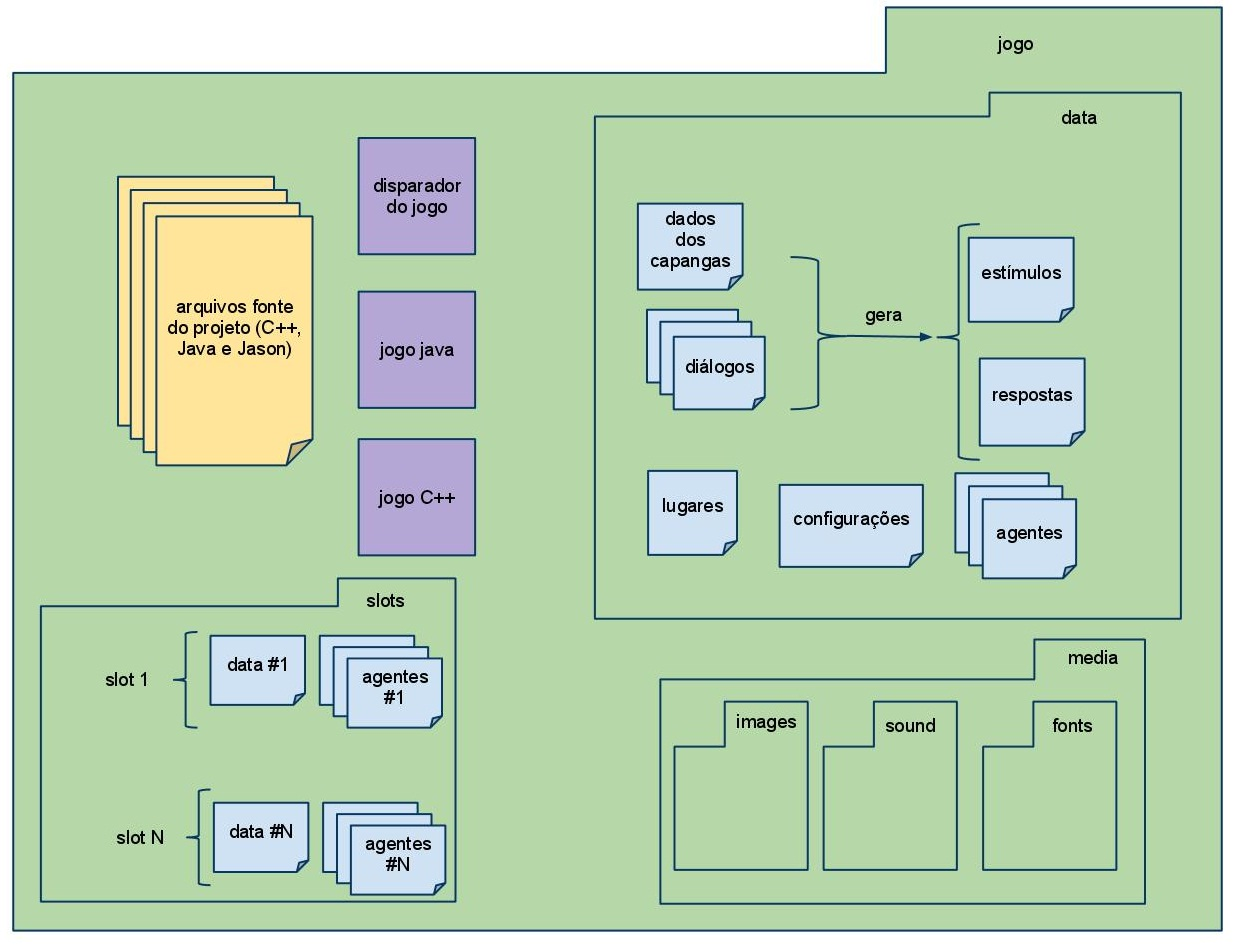
\includegraphics[width=\textwidth]{figuras/estrutura-arquivos.jpg}
\caption{Organização de arquivos do projeto}
\label{fig:estrut-arquiv}
\end{figure}


\section{Arquivos auxiliares}

Uma série de arquivos de texto auxiliares são usados pelo jogo. São em sua maioria estáticos, sendo que alguns são lidos por ambos os programas. Ressalta-se que os conjuntos de arquivos gerados por Java e C++ não têm intersecção, o que elimina a necessidade de gerência de situações de escrita concorrente. Eles especificam:
\begin{itemize}
\item diálogos,
\item modelos de agentes,
\item informações de instâncias de agentes,
\item tipos de reações,
\item tipos de estímulos a agentes,
\item lugares passíveis de assalto,
\item dados de capangas,
\item ações da polícia.
\end{itemize}

Explicamos a seguir a função de cada um dos tipos de arquivo.

Os \emph{modelos de agentes} são arquivos de texto para controle das informações de cada agente. Possuem as seguintes informações sobre os agentes:
\begin{itemize}
\item tipo do agente: inteiro que define o tipo do agente (0-capanga,1-civil,2-policial,3-oculto).
\item id do agente: inteiro único, entre 10 e 99 que representa o agente.
\item nome do agente: String com o nome do agente.
\item personalidade: String que define a personalidade atual do agente.
\item estado psicologico: String que define o estado psicológico atual do agente.
\end{itemize}
Os itens listados acima são comuns a todos os tipos de agentes.
Além dos itens listados acima, os arquivos de agentes policiais possuem uma informação extra sobre a variável \emph{conduta} associada a cada policial, que é uma String que pode assumir dois valores (ganancioso ou íntegro), e os arquivos de agentes capangas possui a variável \emph{nível de suspeita} que é um inteiro (o valor máximo desta variável é definido no arquivo de configuração), ela serve para a polícia monitorar os capangas e decidir se deve ou não prendê-lo.
Vale citar que existe um arquivo por agente e que o nome do arquivo é sempre formado pela seguinte regra: \verb!a! + \verb!tipo-do-agente! + \verb!id-do-agente.txt!

Os \emph{tipos de estímulos, tipos de reações, lugares passíveis de assalto, dados de capangas,} e \emph{ações da polícia} são arquivos de interface, lidos por ambos os programas na decodificação de mensagens trocadas. Optou-se por essa solução para que a comunicação se desse pelo envio de inteiros, indicando qual a linha do arquivo de interface
em que a mensagem está contida. Com isso o processo de alteração do protocolo em seus estágios iniciais de desenvolvimento foi simplificado, uma vez que sua própria especificação atua como um tipo de documentação; além disso, a mudança das mensagens do protocolo passou a ser feita pela mudança de algumas linhas em um arquivo de configuração e em um mapa de strings a funções, o que facilitou a experimentação. Claramente, essa abordagem só é
possível porque as mensagens são conhecidas \emph{a priori}.

Para comunicar o estímulo que uma determinada fala no diálogo provoca
no agente, a lógica do jogo envia ao sistema BDI um inteiro indicando
a linha em que está escrita a string que define o estado. Na prática,
a lógica do jogo faz uma chamada para enviar o inteiro correspondente
ao estímulo que se deseja comunicar, e uma busca é feita no arquivo
que contém os estímulos possíveis para encontrar o conteúdo da linha
correspondente. Essa string é, por fim, enviada ao sistema BDI, que
fará a sua própria busca para identificar qual o estímulo recebido.

Vale notar que os arquivos contendo os estímulos e reações são gerados por um programa que os extrai dos diálogos escritos para o jogo.

Os \emph{diálogos} são scripts que codificam possíveis dizeres que
\npc{}s ou o jogador podem efetuar em um diálogo. Carregam informação sobre
o sentimento que expressam ou a impressão que causam. 
O grupo desenvolveu uma gramática de scripts específica para os diálogos.

\subsection{Cenas e \emph{scripts} de diálogos}
Scripts, em geral, constituem parte da interface entre os times de
desenvolvimento, arte e dessign de games. Muito se discute, nesse
meio, quanta complexidade é interessante que os programadores deixem
acessível por meio do script que criaram. Complexidade em demasia via
de regra vem acompanhada de estruturas elaboradas de programação, com
duas consequências negativas que vale a pena citar
\begin{itemize}
\item aumento no tempo gasto implementando o interpretador de scripts,
\item risco de ocorrer delegação de tarefas da equipe de
  desenvolvimento para as demais.
\end{itemize}

É certo que, usados com parcimônia, os scripts são uma ferramenta
fundamental na dinamização do processo de testes e experimentação
durante a confecção do jogo, e o resultado, é o que alguns chamam
de~\emph{design orientado a dados}, ou~(\emph{data-driven design}).

Nesta seção abordamos duas linguagens de scripts feitas, para controle
de ``filmes'' exibidos durante o jogo, e para composição de diálogos.

\subsubsection{Script de cenas}

Adoou-se uma simplificação no tipo de cena que seria o jogo
comportaria. As cenas são uma sequência de imagens e texto,
acompanhadsd de música --- algo similar a apresentações de slides. Eis
um pequeno exemplo de script.

{\centering
\footnotesize
\begin{verbatim}
<music=musica-de-fundo.mp3>
<background=imagem-de-fundo-1.jpg>
<>Uma ideia brilhante
<wait=1000>
<>Uma ideia brilhante.
<wait=1000>
<>Uma ideia brilhante..
<wait=1000>
<>Uma ideia brilhante...
<wait=2000>
<fadeOut=500>
<background=imagem-de-fundo-2.jpg>
<fadeIn=100>
<>Um projeto
<wait=1000>
<>Um projeto re
<wait=600>
<>Um projeto revo
<wait=600>
<>Um projeto revolu
<wait=300>
<>Um projeto revolucio
<wait=600>
<>Um projeto revolucioná
<wait=600>
<>Um projeto revolucionário!
<wait=2000>
<fadeOut=2000>
<background-color=black>
<>Porém...
<fadeIn=500>
<wait=4500>
<fadeOut>
\end{verbatim}
}

O exemplo acima foi construído para exibir as principais
características do script feito. Primeiro, inicia uma música de fundo,
acompanhada de uma imagem ao fundo. A seguir, uma sequência de frases
é exibida, de modo que fique a impressão de que letras são adicionadas
pouco a pouco. A seguir a tela escurece, prepara-se uma outra imagem
de fundo para substituir a anterior, e o mesmo efeito de substituição
do texto por um texto parecido é empregado para enfatizar a palavra
``revolucionário'', que aparece sílaba por sílaba, a intervalos de
$600$ milisegundos. A tela então escurece novamente, e prepara-se a
exibição de uma tela preta com os dizeres ``Porém\ldots'', que então
aparecem em umatransição de $500$ms. Por fim, após $4,5$ segundos a
tela escurece novamente e a cena termina.

\subsubsection{Script de diálogos}
Descrevemos a seguir a gramática da linguagem de especificação de diálogos.
Os diálogos são criados através de uma linguagem de marcação muito parecida com a linguagem \emph{xml}. Todas as instruções são descritas no começo da linha na seguinte forma: \emph{$<$instrucao1 instrucao2 … instrucaoN$>$ texto}. Vale citar que uma fala pode não ser precedida por nenhuma instrução, representada por \emph{$<>$}, nesse caso a fala, seja ela do jogador ou do \npc{} é simplesmente apresentada. A marcação de fim do diálogo é feita através da sequência $<$/$>$.
Cada diálogo é completamente escrito em um arquivo, sendo assim, quando o jogador inicia um diálogo, somente um arquivo é utilizado e neste arquivo, a primeira fala será sempre a do jogador.

A grande funcionalidade da linguagem criada é que ela oferece, de forma simples opções de falas tanto para o jogador quanto para o \npc{}. Toda vez que for encontrada a sequência \emph{$<$opts$>$} significa que foi aberta uma parte do diálogo é possível ao jogador ou ao \npc{} escolher mais de uma fala. As opções são listadas ao lado da sequência \emph{$<$op$>$}, e ao final da lista de opções deve existir a sequência de fechamento \emph{$<$/opts$>$}.

Outro aspecto interessante da linguagem desenvolvida é a existência de desvios no rumo do diálogo, o desenvolvedor pode dividir o arquivo em blocos de um mesmo diálogo separados por \emph{labels}, como por exemplo, \emph{$<$label sucesso$>$ . . . $<$/$>$} e desviar o diálogo para este bloco através de uma instrução do tipo \emph{$<$goto=sucesso$>$} onde \emph{``sucesso’’} é um label associado a um bloco do diálogo que só será acessado se o jogador ou o \npc{} selecionar uma fala que contenha a instrução descrita acima.

A principal característica da linguagem desenvolvida é que com ela é possível passar ao \npc{} o estímulo que a fala irá produzir, por exemplo \emph{$<$op elogio$>$ voce é linda!}, com isso o \npc pode considerar possíveis opções de resposta, estas por sua vez estão associadas à reações que são descritas da mesma maneira, por exemplo \emph{$<$op agradecer$>$ obrigado!}. 

Além disso, dois detalhes interessantes foram adicionados, um comando que associa uma cor a uma fala do \npc{} e um comando de liga/desliga que pode ser utilizado por exemplo para habilitar/desabilitar itens para o jogador. O fato da cor associada a fala do \npc{} mudar é interessante pois a cor será um tipo de \emph{feedback} para o jogador ter uma noção de como o \npc{} está se sentindo. O comando tem a seguinte sintaxe: \emph{$<$color=cor$>$}, onde a variável cor pode assumir três valores, green (\npc{} está gostando), yellow (\npc{} está apreensivo) ou red (\npc{} não está gostando), além disso, caso o \npc{} esteja indiferente, nenhuma cor é associada à caixa de texto de sua fala. 

O comando para ligar/desligar é da forma \emph{$<$SWITCHON=x$>$} para ativar qualquer coisa que seja representada pela variável \emph{x} ou {$<$SWITCHOFF=x$>$} para desativar.

O último comando que deve ser apresentado é o comando \emph{$<$only=DadoCapanga$>$texto} onde a variável \emph{DadoCapanga} representa algum atributo descrito no arquivo de modelo do capanga em questão. Desta forma, a fala em questão só estará disponível para o jogador se a condição do comando for verdadeira.

A seguir apresentamos um exemplo de um texto de diálogo entre o jogador e um \npc{}. Neste caso, se o jogador tiver sucesso ele destrava um item, ou até mesmo ganha este item, senão não terá acesso ao item e pode até mesmo ter o nível de suspeita de seu capanga incrementado.
Para facilitar o entendimento, as linhas azuis representam as falas disponíveis ao jogador e as linhas pretas as falas disponíveis ao \npc{}.

{\footnotesize
\begin{verbatim}
<! Diálogo entre homens para liberar sonífero / se tornar suspeito >
<opts>
  <op fala-amigavel>Bom dia, senhor.
  <opts>
    <op> Bom dia.
    <op> Olá.
    <op goto=rabugento rabugento color=yello> Bom dia pra quem?!
    <op goto=rabugento rabugento color=yellow> Hmpf, o que o senhor quer?
    <op apressado> Desculpe, estou sem tempo para conversar.
    </>
  </opts>
  <op insulto>E aí véio?
  <goto=retratacao color=red effect=shaking>Quem é velho?
  <op only=EngProd  fala-amigavel elogio>Está um belo dia hoje não?
  Tão belo quanto o senhor!
</opts>

<opts>
  <op inquisitivo>Você trabalha aqui?
  <opts>
    <op goto=sonifero> Não, trabalho na farmácia!
		
		<op goto=sonifero>Não, sou farmacêutico!
		<op apreensivo color=yellow> Por que você quer saber?
	</opts>
<op>Você tem horas?
<>Erm, não...
</>
</opts>
</>
<label retratacao>
<opts>
	<op insulto>Não ouviu? Eu disse E AÍ SURDO!?
	<opts>
<op color=red> Que absurdo!
	<op irritado color=red>Vá se danar!
</opts>
	</>
	<op>Perdão, pensei que fosse um amigo meu. Mas nossa, vocês
são muito parecidos!
	<opts>
		<op only=EngProd>Curioso, você não é o primeiro a me
dizer isso...
		<>Sério? Seria incrível então se o senhor também
trabalhasse com...
		<>Farmácia?
		<>Caramba, isso é que é coincidência! Por falar nisso,
eu estava indo para uma agora...
		<>Doente, por algum acaso?
		<>Bom, não exatamente. Insônia. Faz duas semanas que
eu não consigo dormir direito.
		<switchOn=dormeflex goto=terminabem color=green>Já
sofri disso, é um incômodo. Aceita uma sugestão? Use o  "dormeflex",
vende na farmácia aqui perto.
		<op>Pois é... bom, tchau!
</>
	</opts>

<label sonifero>
<opts>
	<op only=EngProd elogio> Sério? Você caiu do céu!! Você não
teria um remédio para me ajudar a dormir teria?? Tenho sofrido muito
com essa insonia!
	<opts>
	<op goto=enecrraBem feliz SWITCHON=dormeflex color=green>
Claro! 			Também sofro com este problema! Na verdade,
tenho uma pílula aqui no 			bolso, pode levar!!
<op goto=encerraBem  lisonjeado SWITCHON=dormeflex color=green>
Caí do céu?? Que isso, foi pura coincidência! Mas  eu tenho o  remédio
que você precisa, te vendo por um precinho amigo! quer comprar?
<op goto=encerraBem SWITCHON=dormeflex color=green>
Certamente! Passe no mercado e compre um "dormeflex"!
</opts>
	<op suspeito> O senhor vende remédios para fazer alguem
dormir?
	<opts>
		<op apreensivo color=yellow> Claro que sim! Mas por
que o senhor 				desejaria fazer alguém dormir?
<op goto=encerraBem SWITCHON=dormeflex color=green> Vendo sim!
Passe no mercado e compre uma pílula de "dormeflex"! Derruba
elefantes!
</opts>
	<opts>
	<op insulto> Não lhe interessa!
	<op insulto> Pra "alguém" dormir!
	<op fala-amigavel> É para minha esposa! Ela sofre de insônia!
	<op only=EngProd inquestionavel> Vou ser sincero! É para minha
esposa, amanhã tem final do futebol! Preciso que ela durma senão não
posso ver o jogo em paz!!
</opts>
	<opts>
	<op goto=encerraBem SWITCHON=dormeflex compreensivo
color=green> Muito justo o seu motivo! Aqui está, coloque na
bebida dela ou na comida e ela vai dormir a noite toda!
	<op goto=encerraMau color=red> Que absurdo! O senhor quer
drogar sua própria esposa?! Não posso e nem quero participar
disto!
</opts>
	
	<op insulto> Ou, descola uns remédios para dormir pra mim??
		<opts>
			<op goto=encerraMau zangado color=red>  De
jeito nenhum!
			<op goto=encerraMau rabugento color=red> Não
sou traficante 					"mano"!
			<op goto=encerraBem SWITCHON=dormeflex
color=green> 					Compra lá no mercado
uns "dormeflex".
</opts>
</opts>
</>

<label encerraBem>
<! fala do jogador>
	<opts>
		<op fala-amigavel> Muito obrigado!
		<op elogio> O senhor salvou minha vida!! Obrigado!
</opts>
<color=green> Que isso!? É um prazer ajudar! Me procure sempre que
precisar! Até mais!
</>

<label encerraMau>
	<opts>
		<op insulto> Muito obrigado! Por não me ajudar em nada!
		<op fala-amigavel> Desculpe incomodá-lo!
</opts>
<opts>
	<op educado> Sinto muito! Não posso ajudá-lo!
	<op zangado color=red> Veremos o que a polícia acha disso?
	<op apreensivo color=red> Não quero nada com isso!!
	<op> Adeus senhor!
</opts>
</>
\end{verbatim}
}



\chapter{Testes}


Os testes foram concebidos de modo a englobar pequenas histórias de
uso, de um lado, e funcionalidades, de outro.

Os testes planejados de carga e salvamento de progresso foram suprimidos do projeto em razão de sua baixa prioridade quando comparados aos demais testes.

\section{Diálogos}

Este teste envolveu diversos subsistemas do projeto simultaneamente. não apenas o mecanismo de exibição de diálogo, como também o funcionamento da sequência do script de diálogo e as mudanças de crenças dos agentes do BDI foram testados conjuntamente. Estes sistemas haviam sido testados por si, independentemente, mas optou-se por apresentar neste documento uma pequena quantidade de testes significativos da correta operação dos sistemas.

\section{Navegação pelo jogo}

O teste de navegação incluiu a escolha das diferentes opções em cada uma das telas do jogo.

\section{Cenas}

Analogamente aos diálogos, foram testadas diversas cenas do jogo, embora nem todas sejam de fato parte integrante de sua versão final. Os testes ``extras'' tiveram por objetivo testar as funcionalidades implementada da linguagem script de cenas. (Nem todos os comandos previstos são usados nas cenas de fato produzidas para demonstração do projeto.)

\section{BDI em ação}
Este teste foi efeuado juntamente com o teste de diálogos. A ferramenta Jason oferece um recurso de monitoramento da base de crenças e intenções do agente (figura \ref{debug}), com isso, fomos capazes de apresentar todas as alterações que ocorreram nessa base durante um diálogo.
\begin{figure}
\centering
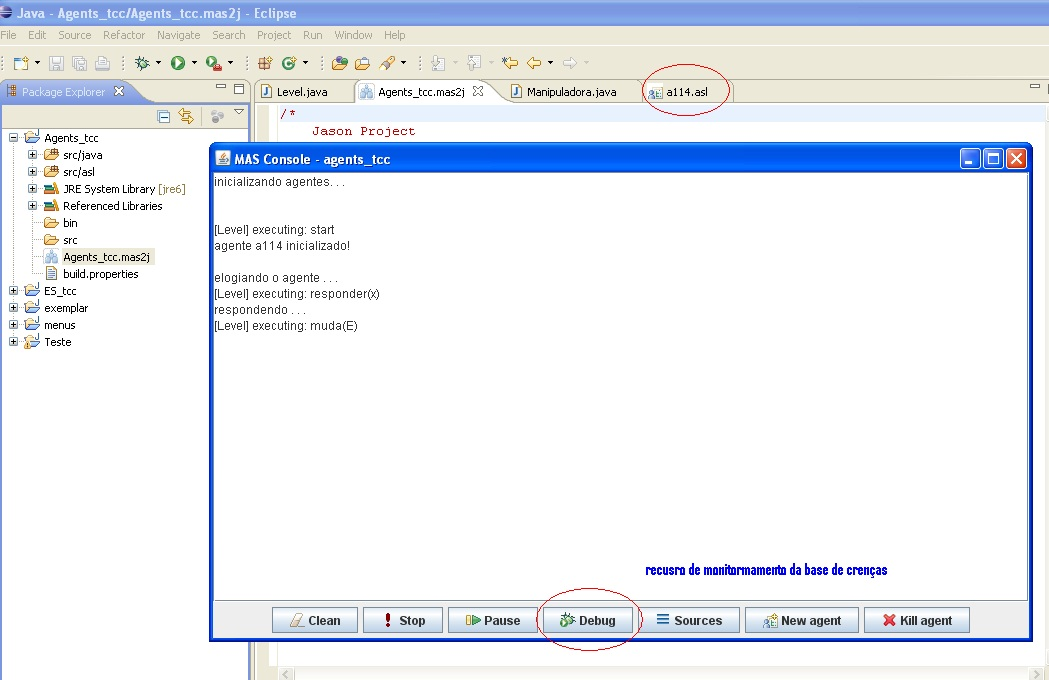
\includegraphics [height=10cm]{figuras/rodando_elogio_jose.jpg}
\caption{Recurso de monitoramento da base de crenças de agentes}
\label{debug}
\end{figure}

A seguir apresentamos uma pequena demonstração de como o agente altera seu estado psicológico em função de um estímulo.
Temos um agente do tipo civil, cuja personalidade foi definida como simpático e o estado psicológico foi definido como feliz, este agente recebeu um estímulo do tipo elogio, como era de se esperar, um agente simpático e feliz continuou simpático e ficou lisonjeado. Apresentamos abaixo o arquivo de modelo do agente antes (figura \ref{ze_antes}) e depois do elogio (figura \ref{ze_depois}) bem como sua base de crenças quando foi elogiado (figura \ref{base_crencas}).

\begin{figure}
\centering
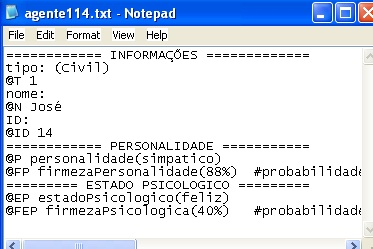
\includegraphics [height=10cm]{figuras/jose_antes.jpg}
\caption{Arquivo de modelo do agente antes do estimulo}
\label{ze_antes}
\end{figure}

\begin{figure}
\centering
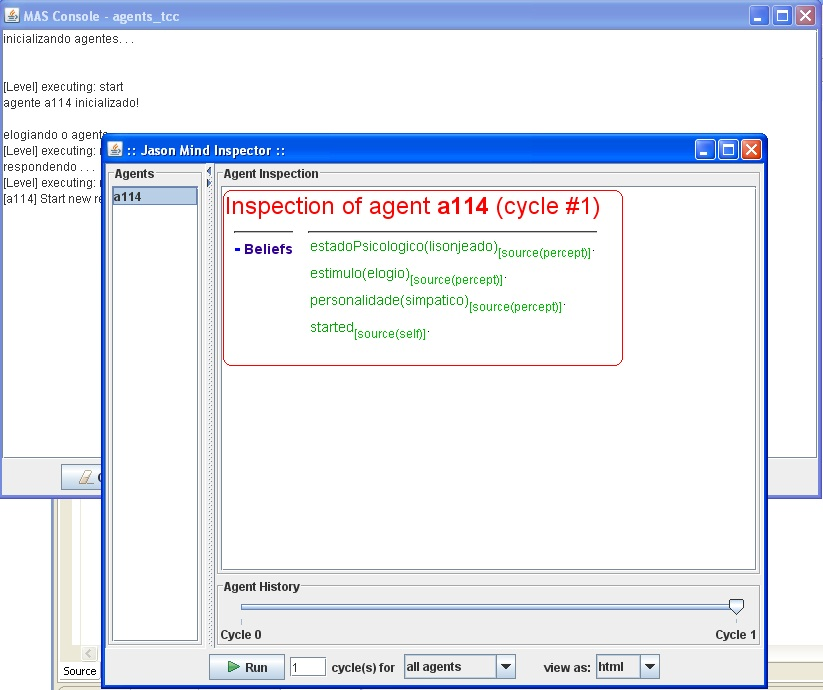
\includegraphics [height=10cm]{figuras/base_crencas_jose.jpg}
\caption{Base de crenças do agente no momento do estímulo}
\label{base_crencas}
\end{figure}

\begin{figure}
\centering
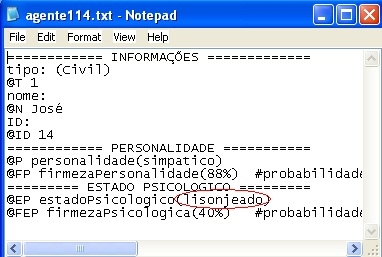
\includegraphics [height=10cm]{figuras/jose_depois.jpg}
\caption{Arquivo de modelo do agente depois do estimulo}
\label{ze_depois}
\end{figure}


\section{Inferência pelo Blackboard}
Da mesma forma que o teste anterior, utilizando o recurso de monitoração da base de crenças dos agentes, observamos o que aconteceu na base dos agentes ocultos quando uma informação foi adicionada por um agente policial.
Como foi explicado no capítulo anterior, existem agentes ocultos da polícia que fazem o processamento das informações enviadas peloas agentes policiais. As informações podem ser dos seguintes tipos(onde P = pessoa e L = lugar):
\begin{itemize}
\item P fez compra suspeita
\item P agiu de modo suspeito em L
\item L foi roubado com sucesso
\item L foi roubado sem sucesso
\end{itemize}
Quando um policial envia alguma das informações acima, ela é repassada a todos os agentes ocultos, no entanto, só alguns sabem processar a informação e geram novas informações que somente outros sabem processar e este processo continua até uma ou mais ações policiais serem geradas.
Dentre as ações que podem ser geradas temos:
\begin{itemize}
\item aumentar nivel suspeita de P
\item diminuir nivel suspeita de P
\item prender P
\item aumentar nivel segurança de L
\item diminuir nivel segurança L 
\end{itemize}
No teste realizado, um capanga (o agente a301) realizou uma atividade suspeita no banco. Um policial reportou aos agentes ocultos estas informações, e o agente oculto (policial a251) concluiu que o nível de suspeita do capanga deveria ser aumentado e o agente oculto (policial a252) concluiu que o nível de segurança do banco deveria ser aumentado, além disso, o nível de suspeita do capanga chegou em um nível tão alto que o agente (policial a255) decidiu decretar sua prisão.

\chapter{Conclusão}

Findo o projeto, resta uma série de considerações a serem feitas,
relativas a diversas dimensões do trabalho desenvolvido. No que
segue, procuramos abordar algumas das questões que foram investigadas,
assim como as que foram surgiram e eventualmente foram deixadas à
margem.

É nossa esperança que esta retomada permita ao leitor vislumbrar um
pouco do fascínio e curiosidade que esses assuntos nos provocaram, e
que, parte delas se espalhe, viceje e reproduza, suscitando sempre
novos questionamentos.

\section{Viabilidade}

No que concerne à aplicação da arquitetura BDI e do blackboard,
chegamos à conclusão de que existem restrições a seu uso. Restrições
em ao menos dois aspectos: conceitual e técnico.

Como discutido na seção~\ref{sec:tradeoffs}, foi observado, com
vantagem para o projeto, o compromisso de limitação da ação
``independente'' do BDI em prol do ganho de controle na composição dos
diálogos. Quanto ao blackboard, existe ainda a questão de encontrar
uma abordagem mais adequada do problema de compartilhamento de
informação. Nosso modelo, simplificado, permitiu avaliar seu
desempenho em quando usado topicamente, o que ainda está longe de
fornecer uma direção de pesquisa em que investigar sua interação com
redes médias e grandes de contextos intersectantes.

De todo modo, observou-se um enriquecimento das possibilidades de
expressão ao se permitir que \npc{}s variem seu comportamento.

Dadas as restrições do projeto, acreditamos que a investigação feita aponta para um resultado promissor, em que técnicas de inteligência artificial permitirão expandir as fronteiras da interação em jogos.

\section{Trabalhos futuros}

Foi identificada uma certa carência de ferramentas de desenvolvimento no decorrer do projeto.
Como a proposta do trabalho foi, de certa forma inovadora, esta carência não foi inesperada. Um caso que se destaca é a falta de ergonomia do método de composição de diálogos que se empregou. Isso pois como tanto o jogador como o \npc{} possuem mais de uma fala possível em alguns nós do diálogo, a árvore de interações possíveis expande rapidamente. Seria interessante desenvolver alguma interface para a  edição desses diálogos, permitindo rápida identificação do locutor, bifurcações e reuniões de linhas do discurso.

Ademais, é interessante que se investigue outros modelos de perfis de agentes, explorando mais as capacidades do AgentSpeak, tanto em variabilidade de perfis como em complexidade dos agentes.

%Seria legal um editor de diálogos, e explorar mais a elaboração de
%perfis de agentes (mais variados e mais complexos)
%Sucesso do estudo de caso?


É importante destacar o papel que a aquisição de conhecimento no domínio do projeto --- e com isso referimo-nos tanto ao estudo técnico quanto ao conhecimento adquirido pelo contato com pessoas do ramo --- na mudança da própria maneira e enfoque do projetar e compreender o projeto do jogo. Nesse contexto é notável o papel que desempenhou o curso de uma disciplina do domínio da produção de jogos\footnote{A referida disciplina é Design e Programação de Games  (\textsc{PCS2530}), cursada no segundo semestre de 2010.}, assim como a participação no SBGames, nos quais adiquiriu-se um conhecimento
que, de certo modo, não está acessível por meio das vias consagradas de estudo; um conhecimento vivo, orgânico, da esfera cultural que é parte inerente dos jogos neste tempo.

Muito mais do que estávamos cientes, os jogos digitais encontram-se, hoje, em uma posição
privilegiada, na fronteira entre tecnologia e arte, entre ciência e
cultura. Há toda uma dimensão no jogo, uma dimensão além de um
entretenimento que é produto e passa-tempo apenas. Um universo vasto e cheio de possibilidades a explorar.

É nessa perspectiva que o grupo cogita a possibilidade de continuar o desenvolvimento de projetos na linha de investigação da aplicação de técnicas de inteligência artificial a jogos, com vistas a participar do próximo Simpósio Brasileiro de Games, apresentando os resultados dessa pesquisa.


\addcontentsline{toc}{chapter}{Referências Bibliográficas}
\bibliographystyle{abnt-num}   %\bibliographystyle{plain}
% \bibliography{bibname.bib} % bibname=nome do seu arquivo BibTeX
\begin{thebibliography}{99}
\bibitem{tese_roberto}
    BIANCHINI, R. C. \textbf{Uma arquitetura BDI para comportamentos interativos de agentes em jogos computacionais}. Tese de doutoramento --- Escola Politécnica da Universidade de São Paulo, São Paulo, 2005.

\bibitem{livro_russel}
    NORVIG, P.; RUSSEL, S. \textbf{Inteligência artificial}. 1 ed. São Paulo: Elsevier editora ltda, 2007. ISBN: 978-85-352-2564-8.

\bibitem{brian_schwab}
SCHWAB, B. \textbf{AI game engine programming}. 2 ed. Hingham: Charles River Media, 2008.

\bibitem{wooldrige_agentes}%[4]
WOOLDRIDGE, M. \textbf{Reasoning about rational agents}. Cambridge: The M. I. T. Presss, 2000.

\bibitem{oliveira_BDI}%[5]

NUNES, I. O. \textbf{Implementação do modelo e da arquitetura BDI}. Monografias em Ciência da Computação --- Pontifícia Universidade Católica do Rio de Janeiro, Rio de Janeiro, 2007.
ISSN 0103-9741

\bibitem{design_games}
SCHUYTEMA, P. \textbf{Design de Games: uma abordagem prática}. São Paulo: Editora Cengage, 2008

\bibitem{artigo_turing}
TURING, A.M. \textbf{Computing machinery and intelligence}. Mind, 1950. Disponível em: $<$\url{http://www.loebner.net/Prizef/TuringArticle.html}$>$. Acesso em: 20 ago. 2010.

\bibitem{beejs}
HALL, B. \textbf{Beej’s guide to network programming}: using internet sockets. 2009.Disponível em: $<$\url{http://beej.us/guide/bgnet/output/html/multipage/index.html}$>$.
Acesso em: 30 jul. 2010.

\bibitem{deitel}
DEITEL, H.M.; DEITEL, P. J.\textbf{Java}:como programar. 6 ed. São Paulo: Pearson Prentice Hall, 2005. ISBN: 85-7605-019-6.

\bibitem{jomi}
BORDINI, R.H. et al. \textbf{Programming multi-agent systems in AgentSpeak using Jason}. São Paulo: Wiley, 2007. ISBN: 978-0-470-02900-8

\bibitem{kishimoto}
KISHIMOTO, A. \textbf{Inteligência Artificial em Jogos Eletrônicos}. São Paulo: 2004. Disponível em $<$\url{http://www.programadoresdejogos.com/trab_academicos/andre_kishimoto.pdf}$>$.
Acesso em: 20 set. 2010

\bibitem{AndrewDave-arquitet-e-design}

ROLLINGS, A.; MORRIS, D. \textbf{Game Architecture and Design}. Albany: Coriolis Group Books Editora, 1999. ISBN 0-7357-1363-4.

\bibitem{John-Omar-SwEngForGames}
    FLYNT, J.; SALEM, O. \textbf{Software engineering for game developers}. Boston, MA: Course Technology PTR Editora, 2005. ISBN: 1-59200-155-6.

\bibitem{Steve-AIgameWisdom}
    RABIN, S. \textbf{AI game programming wisdom}. Hingham, Mass.: Charles River Media Editora, 2002. ISBN: 978-1584500773.

\bibitem{design-patterns}

GAMMA, E.; et al. \textbf{Design patterns : elements of reusable object-oriented software} Reading, Mass. : Addison-Wesley Editora, 1995. ISBN: 978-0201633610

\bibitem{thining-cpp}
    ECKEL, B. \textbf{Thinking in C++}. Upper Saddle River (N. J.) : Prentice Hall Editora. 2000. ISBN: 978-0139798092.

\bibitem{accel-cpp}
    KOENIG, A.; MOO, B. E. \textbf{Accelerated C++ : practical programming by example}. Boston, MA : Addison-Wesley Editora, 2000. ISBN: 978-0201703535.

\bibitem{Julien-oogd}
    GOLD, J. \textbf{Object-oriented game development}.Harlow, England ; New York : Addison Wesley Editora, 2004. ISBN: 978-0321176608
\bibitem{Prog-Linux-games}
    HALL, J. R. Loki Software Inc. \textbf{Programming Linux Games}.San Francisco: No Starch Press, 2001.ISBN: 978-1886411494.
 
\end{thebibliography}


\addcontentsline{toc}{chapter}{Glossário}
%\include{capitulos/glossario}

% anexos (opcional)
\addcontentsline{toc}{chapter}{\appendixname}
\appendix
%\chapter{Gramática dos \emph{scripts} de
  diálogo}\label{ap:gram-script-dialogo}

Descrevemos a seguir a gramática da linguagem de especificação de diálogos.


%\chapter{Protocolo de comunicação entre C++ e Java}\label{ap:protocolo}

A necessidade de comunicação entre os subsistemas de processamento da inteligência articial implementada e os mecanismos de controle e renderização do jogo surgiram tão logo se foram definidos dois requisitos do projeto, em seu início: o emprego de C++, de modo a refletir um padrão amplamente empregado na indústria de jogos, e a opção pelo uso do interpretador de AgentSpeak, Jason, que possui apenas interfaces para Java.

Definiu-se então um protocolo simples, operando via TCP (\emph{loopback}), o que não incorre em perdas significativas de eficiência na troca de informações. O protocolo, que passou por diversas modificações ao longo da evolução do projeto, baseia-se na troca de mensagens, sequencias de inteiros, que respeitam regras simples:
\begin{enumerate}
\item o primeiro inteiro enviado representa quantos inteiros mais compõe a mensagem;
\item o segundo inteiro identifica o nome da mensagem;
\item os demais inteiros são parâmetros da mensagem.
\end{enumerate}

O nome da mensagem é recuperado pelo receptor da mensagem pela leitura de um arquivo de referência --- é a linha de número igual ao inteiro recebido. Munido dessa cadeia de caracteres, o receptor então pode buscar em um mapa interno a função responsável por tratar a mensagem e seus argumentos. De modo análogo, os argumentos representam, na maior parte das vezes, o número da linha que deve ser lida em algum arquivo do sistema (pré-definido para cada nome de mensagem) contendo algum complemento da informação.

\section{Arquivos consultados}

Os arquivos que são lidos pelas rotinas de tratamento das mensagens são
\begin{description}
\item[estímulos] contém estímulos que podem ser enviados a agentes no decorrer de diálogos;
\item[respostas] contém as respostas que agentes podem expressar em diálogos;
\item[capangas] contém nome (e possivelmente outras informações) a respeito de capangas na equipe dos \nomeGrupo;
\item[lugares] contém o nome de lugares passíveis de roubo;
\item[predicados] contém uma lista de avisos que podem ser dados à polícia;
\item[configurações] contém, respectivamente, em suas linhas
\begin{enumerate}
\item o número da porta de comunicação loopback empregado pelos subsistemas em sua comunicação;
\item o número de slots que o jogo possui
\item o maior nível de suspeita possível para capangas (que é também o maior nível de segurança para lugares)
\end{enumerate}
\end{description}

\section{As mensagens}

O conjunto de mensagens passou por várias alterações desde sua primeira concepção, o que não somente era esperado, como demonstrou a utilidade da arquitetura de troca de mensagens que havia sido projetada, preparada para acomodar sem grande dificuldade adições e remoções de mensagens. As mensagens são listadas a seguir.

\begin{enumerate}\footnotesize
\item \verb!iniciaDialogo( )! solicita o envio do id de um agente com
  quem o jogador está iniciando um diálogo (o perfil e estado
  psicológico do agente são sorteados pelo subsistema Java);
\item \verb!retornaIdAgente()! retorna um id solicitado por \verb!iniciaDialogo()!;
%
\item \verb!estimuloagente ( # agente, # estímulo )! estimula o agente
  referido;
%\item \verb!atualizaBeliefs(# agente, # estimulo)! 
%
\item \verb!ofereceEscolhas( # agente, # reacao1, # reacao2, … )!
 lista uma série de reações que o agente pode expressar;
\item \verb!returnEscolha(# agente, #escolha)! retorna a escolha
  escolhida pelo agente como a que mais se aproxima de expressar seu
  estado psicológico atual;
%
%
\item \verb!fimDialogo( #agente )! avisa o término do diálogo;
\item \verb!acaoDaPolicia( #acao, #alvo )! solicita ao jogo que tome
  alguma ação em nome da polícia; ações previstas incluem
  \begin{itemize} 
  \item  aumentar nivel suspeita de capanga (alvo);
  \item  diminuir nivel suspeita de capanga (alvo);
  \item  prender  capanga (alvo);
  \item  aumentar nivel segurança de lugar (alvo);
  \item  diminuir nivel segurança de lugar (alvo);
  \end{itemize}
%
\item \verb!avisaPolicia( #sujeito, #predicado )! informa a polícia de
  algo:
  \begin{itemize}
  \item alguém fez compra suspeita;
    \item tentativa de roubo (sucesso);
      \item tentativa de roubo (sucesso);
  \end{itemize}
\item \verb!avisaPolicia( #sujeito, #predicado, #alvo )! informa a
  polícia de algo sobre alguém;
  \begin{itemize}
  \item alguém agiu de modo suspeito em um dado lugar;
  \end{itemize}
%[10 escreveBlackBoard(#sujeito, #predicado)] => 8
%
\item \verb!loadGame(! \#slot \verb!)! solicita carga de jogo;
\item \verb!newGame(! \#slot \verb!)! solicita novo jogo;
\item \verb!saveGame(! \#slot \verb!)! sollicita salvamento de jogo
\item \verb!quitGame()! informa fim de jogo.
\end{enumerate}

\begin{comment}
0 - “número de números”
1 - tipo de mensagem
2 … - parâmetros

EXEMPLOS DE ARQUIVOS DE CONSULTA

capangas:
joe
josé
ricardo
arroz
roney
antônio

estímulos:
oferece-propina
fala-amigavel
elogio
insulto
fala-timida

reações:
aceita-propina
rejeita-propina
insultar
elogiar
agradecer

lugares:
oficina mecânica (QG),
mercado,
loja de importados,
loja de carros,
banco, e
joalheria.

configurações:




\end{comment}


\chapter{Game Design Document}\label{ap:gdd}
\section{Visão geral essencial}
%A principal função da primeira seção do documento é fazer com que qualquer pessoa se familiarize rapidamente com a idéia do jogo, o que o fará se destacar e --- ter boa jogabilidade.

Em ``crimechanics'' o jogador deve arquitetar diversos roubos em uma cidade controlando uma gangue de engenheiros, cada um com suas habilidades específicas. O jogador deve fazer o reconhecimento dos alvos, conversar com personagens para coletar informações sobre o alvo e comprar itens para sua equipe. No entanto, é preciso ter cautela, a polícia já foi avisada e fará o possível para evitar os roubos.

\subsection{Resumo}
%O resumo é uma síntese de toda a experiência do jogo.

A interação com o jogo se dá principalmente  por meio de diálogos e menus. Assim o jogador compra itens, estuda a segurança dos lugares que pretende roubar, gerencia a equipe a participar de cada investida e também os dividendos dos participantes.

\subsection{Aspectos fundamentais}
%O objetivo desta seção é extrair componetes fundamentais do jogo que constituirão a trama central para a experiência e a diversão do jogador.

\newcommand{\nomeCidade}{Cobrópolis}

O jogo narra a história de um grupo de engenheiros, cujo líder é controlado pelo jogador, que planejam subverter a ordem do poder local. A cidade é uma cidade planejada pelos próprios engenheiros, para ser um ambiente sustentável e um modelo de igualdade social. Acontece que um dos maiores investidores do projeto, o dr. Pinheirótopos, mudou as regras do jogo perto do fim, e, mostrando-se um prefeito despótico ao assumir o cargo, proibiu o exercício de engenharia no perímetro da cidade. Além disso, transformou-a num paraíso para abastados, decidindo pelo número de dígitos no saldo da conta bancária os cidadãos que teriam direito a viver em \nomeCidade.

Com o intuito de esvaziar a cidade, e esvaziar o poder do autoproclamado prefeito Pinheirótopos, o grupo de projetistas da cidade se organiza clandestinamente e passa a planejar roubos, desacreditando a segurança que eles mesmos haviam concebido para a cidade.

\newcommand{\nomeGrupo}{Crimechanics}

Sem emprego, e revoltados com o rumo dos acontecimentos, o grupo ilegal de engenheiros se forma: os \nomeGrupo{} se preparam para uma batalha épica contra o prefeito.

\subsection{Golden nuggets}
Na concepção da inteligência artificial do jogo foi empregada a arquitetura BDI para agentes, com a finalidade de torná-los mais realistas e adaptáveis do que simples máquinas de estados. Com isso, a interação do usuário com os \npc{}s será muito mais rica, pois o rumo de um diálogo passa a ser mais imprevisível.

\section{Contexto do jogo}
\subsection{História}

Há muitos anos um homem, doutor Pinheirótopos convenceu diversos colegas, todos eles engenheiros, a investirem muito tempo e muito dinheiro em um projeto para fundar uma cidade onde pessoas mais pobres teriam acesso a educação e saúde e poderiam levar uma vida digna. Os engenheiros perderam muitas noites de sono desenhando plantas de edifícios e desenvolvendo sistemas para melhorar a qualidade de vida das pessoas que lá habitariam.
No entanto, Pinheirótopos deu um golpe, elegeu-se prefeito da cidade, e mostrou suas verdadeiras intenções: aumentou impostos, criando com isso uma barreira para justo aqueles para quem a cidade havia sido projetada; os cidadãos que não conseguiam pagar a vida na cidade foram deslocados para periferias e separados da cidade pela polícia.

Pinheirótopos ficou muito rico e transformou a pequena cidade em um pequeno império, em que apenas pessoas selecionadas  por ele poderiam morar. Deu preferência a amigos, conhecidos e àqueles que sabiam agradá-lo. Detém total controle da cidade, afinal (sic) fora projetada por engenheiros, devido a um avançado sistema de segurança, com câmeras espalhadas pelas ruas monitorando a movimentação na cidade 24 horas por dia, e um sistema de alarmes em todos os edifícios que se comunica diretamente com a sede da polícia. Além disso, Pinheirótopos proibiu o emprego de engenheiros na cidade. Esta lei absurda nasceu de uma rivalidade universitária de sua juventude, que o prefeito havia ocultado por longos anos.

Na periferia da cidade, os engenheiros que construíram este sonho se uniram e agora estão dispostos a recuperar a cidade das mãos deste poderoso e inescrupuloso homem. Para isso, a solução encontrada foi deixar a população seleta de Pinheirótopos insatisfeita com o lugar e seu regente. Os engenheiros se organizaram e montaram uma “gangue”, os \nomeGrupo{}, que roubará os melhores estabelecimentos da cidade para enfraquecer a economia da cidade e mostrar que ninguém está seguro e nem protegido como sempre garantiu Pinheirótopos.

%\subsection{Eventos anteriores}
%Esta seção explica o contexto da história do jogo. Dependendo da simplicidade do projeto %pode ser vazia.


\subsection{Principais jogadores}
%Se no projeto do jogo os personagens forem elementos-chave, nesta seção devem ser apresentados e explicados os principais personagens do jogo.

O jogador controla um personagem que gerencia as atividades dos \nomeGrupo. Ele é um engenheiro, mas especialidade é desconhecida, e seu papel no grupo é coordenar, muito mais do que executar os roubos propriamente ditos.

\section{Objetos essenciais do jogo}

\subsection{Personagens}
%Esta seção descreve os personagens do jogo, desde os principais personagens envolvidos na histório da jogo aos \npc{}s aliados ou inimigos menos importantes.


Os personagens do jogo estão divididos em três classes: civis, policiais e capangas.

Os civis são agentes que estão espalhados nos níveis do jogo, o jogador pode iniciar diálogos com qualquer civil presente e dependendo do desenrolar da conversa pode conseguir informações sobre determinados alvos ou mesmo desbloquear itens, que passam a poder ser comprados (ou até mesmo conquistados) e usados nos roubos.

Os policiais são agentes espalhados nos níveis do jogo que observam as ações ao seu redor e reportam à central da polícia qualquer atividade que considerem suspeita. Além disso, podem efetuar prisões de capangas. O jogador também pode iniciar diálogos com um policial e num caso de sucesso pode tentar suborná-lo e descobrir informações importantes sobre o processo de investigação da polícia. Além disso, existem agentes policiais que são ocultos ao jogador, estes agentes são responsáveis pelo processamento das informações no blackboard.

Os capangas que compõem a gangue também são agentes, a maior diferença em relação aos outros tipos de agentes é que todos os capangas possuem uma mesma lista de habilidades. A especialidade de cada um (elétrico, computação, produção, químico, mecânico ou civil) influencia diretamente em seu desempenho em tarefas específicas.
Todos os personagens são agentes criados utilizando a arquitetura BDI.

\subsubsection{Lista de habilidades}
\begin{table}\footnotesize
\begin{tabular}{ccccccc}
& computação & civil & elétrico & mecânico & produção & químico \\
\hline
invadir sistema & 7&2&4&2&2&2\\
reconhecimento de segurança & 3&7&4&4&2&2\\
danificar infra-estrutura &3&7&5&4&2&3\\
desligar aparelhos &6&4&7&3&2&2\\
falsificar crachá &3&4&7&2&6&2\\
arrombar &3&5&4&7&2&4\\
carisma &3&4&2&4&8&5\\
explodir &3&5&3&4&2&7\\
arma química &3&1&1&1&2&7\\
força &4&5&2&7&6&5\\
pontaria &5&5&5&6&5&5\\
\hline
\end{tabular}
\caption{Matriz de habilidades dos capangas.}\label{tab:habilidadesCapang}
\end{table}


\subsection{Características comuns dos agentes}
Todos os agentes possuem ao menos duas características em comum, sua \emph{personalidade} e  \emph{estados psicológicos}. Estas características são importantes pois é graças a elas que os agentes conseguem deliberar durante um diálogo. Elas influenciam diretamente nas ações e respostas do mesmo.

É válido ressaltar a difernça conceitual entre ambas as características. O estado psicológico de um agente pode ser visto como o análogo do estado de um autômato. A principal diferença entre ambos é que as transições de estado psicológico dependem do contexto percebido pelo agente. Além disso, fixados um contexto e uma tendência a alteração do estado psicológico, situação mais detalhada posteriormente nesta seção, o próximo estado psicológico dependerá também da personalidade do agente, que reflete, de certo modo, como o agente reage a estímulos. Note-se que a personalidade não é algo fixo, embora altere-se raramente. Retomando a analogia com autômatos, e expandindo-a de certa forma, é como se personalidades distintas fossem conjuntos de estados próximos entre si, com grande probabilidade de serem visitados em seguida para a maior parte das cadeias. Assim, é improvável que um agente mude de personalidade, enquanto, por outro lado, é provável que vários estados psicológicos associados a uma mesma personalidade sejam visitados durante a operação do agente.


Além disso, existem \emph{estímulos}, que são gerados conforme o jogador opta por determinadas falas durante um diálogo com um agente. O agente recebe então estes estímulos, e varia seu estado psicológico ou até mesmo sua personalidade de acordo com os estímulos recebidos.

\subsubsection{Tipos de personalidades}
Abaixo são listados os possíveis estados psicológicos em que um agente pode estar durante um diálogo. Cada estado psicológico influencia  as decisões do agente de alguma forma.
%-->> Listar as personalidades
\begin{itemize}
\item rabugento
\item simpático
\item educado
\item grosseiro
\item apressado
\end{itemize}

\subsubsection{Tipos de estados psicológicos}
Abaixo são listados os possíveis estados psicológicos em que um agente pode estar durante um diálogo. Cada estado psicológico influencia  as decisões do agente de alguma forma.
%-->> Listar os estados psicológicos
\begin{itemize}
\item feliz
\item zangado
\item apreensivo
\item lisonjeado
\item compreensivo
\end{itemize}

\subsubsection{Tipos de estímulos}
Abaixo são listados os estímulos que são enviados a um agente durante um diálogo conforme as falas que o jogador seleciona.
%Listar os estímulos
\begin{itemize}
\item oferece-propina (Estímulo exclusivo aos agentes policiais)
\item fala-amigavel
\item elogio
\item insulto
\item fala-timida
\item inquisitivo
\item suspeito
\item inquestionavel
\end{itemize}

No caso dos agentes policiais existe uma variável \emph{conduta} que é determinante no caso de um suborno, podendo assumir apenas dois valores.
\begin{itemize}
\item lisonjeado
\item compreensivo
\end{itemize}


\subsection{Armas}
O sucesso de um roubo depende muito das habilidades de cada capanga da gangue. As habilidades são iguais para todos os capangas (ou seja, não existem ``classes'' diferentes), o que varia é o quão bem desenvolvida é a habilidade em cada capanga. Além disso, existem itens que o jogador pode comprar e equipar seus capangas com a finalidade de aumentar o nível de habilidades específicas.

\subsubsection{Lista de itens}

Segue uma lista dos itens disponíveis para compra no mercado do jogo (``Lojas Tem’’, tudo o que você precisa!''), em que são discriminadas pequenas descrições que serão apresentadas ao jogador.

\begin{description}
\item[arma] Use com responsabilidade! [é necessário fazer registro! (ou não)]
\item[picareta] Tool-kit casa dos seus sonhos.
\item[dormeflex] Remédio para adormecer (mamíferos em geral)
\item[bife] O prato favorito dos cães.
\item[chave de fenda] Imprescindível!
\item[maçarico] Tool-kit casa dos seus sonhos. Sabendo usar, abre até cofres!
\item[ácido sulfúrico] Nas mãos certas dissolve tudo!
\item[tnt] Ideal para demolições bem barulhentas
\item[terno] Todo mundo fica bem de terno!
\item[cosméticos] Para embelezar!
\item[alicate] Tool-kit casa dos seus sonhos.
\item[pda] Veja seu email ou jogue tetris na fila de espera!
\item[máscara de carnaval] Ninguém vai te reconhecer!
\item[fralda] Deixe seu bebê sequinho e confortável!
\item[fantasia de ladrão] Máscara, luvas e tudo o mais que um ladrão precisa! (para uma festa!)
\item[Rainequem] Para animar qualquer festa! Beba geladinha!
\item[corta-vidro] Tool-kit casa dos seus sonhos.
\item[hp] Não saia de casa sem a sua.
\item[jornal] Palavras cruzadas!
\end{description}

\subsection{Estruturas}
O jogo acontece em uma cidade fictícia onde existem três tipos estruturas, os alvos que são estabelecimentos que o jogador tentará roubar, o quartel general (chamado de ``oficina mecanica’’) que apresenta a interface de controle da equipe para o jogador poder arquitetar os roubos e o mercado onde o jogador pode comprar itens para equipar seus capangas.
Na tela de apresentação é mostrado um mapa da cidade, numa visão superficial onde o jogador pode clicar em cada estrutura para analisar as opções disponíveis em cada caso.
No caso dos alvos, todos possuem uma variável (interna) associada chamada \emph{nível de segurança} que representa o nível de atenção que a polícia dedica a um determinado alvo, quanto maior o valor da variável maior será o esquema de segurança associado ao lugar e, consequentemente, menores são as chances de um roubo ser bem sucedido.
O valor desta variável é alterado conforme a variação no valor de outra variável, o \emph{nível de suspeita} do local que indica as chances do local ser um alvo segundo a inteligência da polícia.

%-->> Listar os alvos
Os possíveis alvos são os seguintes:
\begin{itemize}
\item loja de importados,
\item loja de carros,
\item banco, e
\item joalheria.
\end{itemize}

%\subsection{Objetos} (NÃO HÁ)

\section{Conflitos e soluções}
No jogo proposto, o adversário do jogador é a polícia. A polícia fará o possível para prender os capangas do jogador e frustrar as tentativas de roubo. A prisão é decretada se o nível de suspeita de um capanga, que é uma variável oculta que a polícia atribui a cada capanga, chegar a um nível muito elevado. Além disso, a polícia pode aumentar o nível de segurança de um alvo se  o valor da variável nível de suspeita do local, que indica as chances do local ser um alvo segundo a inteligência da polícia, chegar a um nível muito alto.

O jogador deve tomar cuidado para não perder capangas, evitando fazer atividades supeitas como reconhecimento e diálogos nos quais o \npc{} com quem esteja conversando se ofenda e tome uma atitude que possa chamar a atenção do policial no cenário.
Um capanga preso fica indisponível, o jogo termina se o jogador perder todos os seus capangas.

Além disso, o jogador pode tentar subornar um policial para descobrir informações sobre os níveis de segurança dos alvos e os níveis de suspeita dos capangas, mundi dessas informações o jogador pode alterar sua estratégia, utilizar outro capanga ou roubar outro alvo. É importante lembrar que um suborno mau sucedido implica na prisão direta do capanga em uso.

\section{Inteligência Artificial}
O uso da arquitetura BDI tem como objetivo melhorar a experiência do jogador, principalmente durante os diálogos.

No jogo em questão todos os \npc{}s são agentes modelados através da arquitetura BDI. Os agentes foram modelados de forma que conforme um diálogo acontece, suas respostas variam de acordo com seu estado interno, e este, por sua vez, varia de acordo com estímulos que são enviados pelo jogador de forma subliminar através dos diálogos, por exemplo, se um agente tem uma personalidade simpática e um estado psicológico feliz e recebe como estímulo do jogador um elogio, seu estado psicológico passa a ser \emph{lisonjeado} e ele provavelmente optará por uma resposta que expresse sua gratidão.

Além disso, foi utilizada uma técnica conhecida como blackboard de solução de problemas de forma cooperativa que é utilizada por agentes da polícia, ocultos ao jogador, que através desta processam informações enviadas pelos agentes policiais das fases.

Um agente policial nota alguma atividade suspeita e envia essa informação para uma base de conhecimento a qual os agentes ocultos possuem acesso. Estes agentes ocultos processam essa informação e podem (ou não) enviar a todos os agentes policiais alguma nova ação que deve ser realizada, tal ação é passada a todos os agentes policiais como um objetivo na arquitetura BDI.
A figura \ref{blackboard_policia} apresenta de forma visual a estrutura descrita acima.
\begin{figure}
\centering
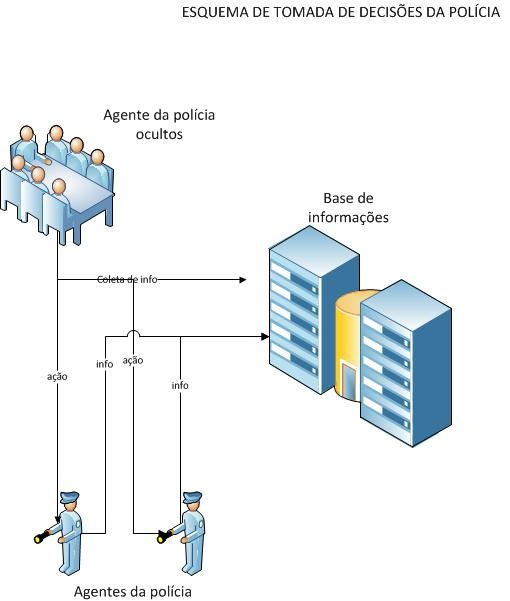
\includegraphics [height=10cm]{figuras/blackboard_policia.jpg}
\caption{Esquema do blackboard no jogo}
\label{blackboard_policia}
\end{figure}

\section{Fluxo do jogo}
%basicamente o guia dos programadores, artistas, designers de níveis e de missões. Aqui devem ser detalhados todos os aspectos de como o jogo funcionará
%De longe a mais longa!

\section{Controles}
Praticamente todo o jogo é baseado no conceito de point-and-click, ou seja, a grande maioria dos controles é feita através do mouse. Exceto durante diálogos quando forem apresentadas diversas opções de fala ao jogador, este selecionará uma fala através do teclado, onde cada fala será representada por um número.

\section{Variações de jogo}
Existem diversas maneiras como um roubo pode ser realizado, o jogador é livre para bolar seu próprio plano. A forma de arquitetar um determinado roubo é sempre a mesma, no entanto, quanto mais o jogador investigar antes da ação e quanto mais itens (pertinentes ao roubo) o jogador utilizar, maiores são as chances do roubo ser bem sucedido.

%\section{Definições}

%\section{Referências}


%\input{capitulos/apendice-A}
%\input{capitulos/apendice-B}

% indice remissivo (opcional)

\end{document}
